\documentclass[12pt,italian]{report}
\usepackage{thesis}

\def\myCDL{Bachelor's Degree in\\Computer Science for Digital Communication}

\def\myTitle{Use Of Deep Learning Techniques for the Reconstruction of Electrocardiographic Signals}

\def\myName{Luca Armetta}
\def\myMat{979049}

\def\myRefereeA{Dr. Massimo Walter Rivolta}
\def\myRefereeB{Prof. Roberto Sassi}

\def\myYY{2022-2023}

\usepackage[a4paper]{geometry}
\usepackage{array}
\usepackage{float}
\usepackage{caption}
\usepackage{subcaption}
\usepackage[english]{babel}
\usepackage[utf8]{inputenc}
\usepackage[a-1b]{pdfx}

\usepackage{graphicx}
\usepackage{hologo}
\usepackage{epsfig}
\usepackage{xcolor}
\usepackage{afterpage}

\newcommand\blankpage{
    \null
    \thispagestyle{empty}
    \addtocounter{page}{-1}
    \newpage}

\usepackage{amssymb,amsmath,amsthm}
\usepackage{listings}
\usepackage{verbatim}

\usepackage{url}
\usepackage[pdfa]{hyperref}

\begin{document}

\afterpage{\blankpage}
\frontespizio
\beforepreface
\afterpreface
\afterpage{\blankpage}

\chapter{Introduction}
\label{chap:introduction}

\section{Electrocardiogram}
\label{sec:electrocardiogram}

Electrocardiography is a very common and non-invasive diagnostic procedure that consists of recording the electrical activity of the heart using electrodes, and its interpretation is increasingly supported by algorithms.

Progress in the field of automatic ECG analysis has so far been hindered by the lack of adequate datasets for network training, as well as the lack of precise and adequate evaluation procedures capable of ensuring the similarity of different algorithms~\cite{deeplearning}.

Standard ECGs consist of 12 leads interpreted as axes through which each ECG records the electrical potentials of the atria and ventricles of the heart. In this type of ECG, four electrodes are placed on the patient's limbs and six on the chest surface, and thus the overall electrical potential of the heart is measured in twelve differences between points, commonly called "leads," and recorded for a predetermined period, usually ten seconds~\cite{ecg}. Two fundamental processes then come into play, known as depolarization and repolarization, which respectively indicate the process by which a cardiac cell changes its electrical state from a negative resting potential to a positive one, and the opposite process, that is, after a cell has depolarized, it must return to its negative resting state to be ready for another electrical impulse. In this way, the overall amplitude and direction of the heart's electrical depolarization are captured at every moment and throughout the cardiac cycle. At the end of repolarization, there is a period of electrical inactivity during which the ECG trace remains isoelectric until the next electrical impulse originates. Therefore, correct interpretation of the ECG is possible with a high-quality 12-lead tracing, and it is advisable to follow a systematic approach that allows proceeding in a predetermined order.

Electrocardiography also allows the detection of many cardiac conditions, including arrhythmias, myocardial infarctions, anomalies of an atrium or a ventricle, coronary artery diseases... but also for continuous monitoring of cardiac patients by recording the heart's electrical activity over an entire day, allowing for a detailed assessment of heart rate variations and the detection of events such as pauses, tachycardias, or bradycardias~\cite{classification}.

Frank leads represent an electrocardiographic acquisition methodology that provides detailed information on the spatial distribution of the heart's electrical activity. The acquisition of Frank leads is non-invasive and can be relatively easily performed using a set of electrodes placed on the patient's chest surface, covering different regions of the heart. Unlike standard 12-lead ECGs, Frank leads allow for a more complete mapping of the heart's electrical activity. This enables a different assessment of the morphology of electrical impulses, as well as cardiac anomalies and disorders.

During the research, Frank leads were implemented due to their important correlation with the three-dimensional X, Y, and Z leads. Since they play a significant role in the analysis of cardiac electrical activity and provide a spatial representation of the heart's electrical activity, Frank leads can be associated with the signals recorded by the X, Y, and Z leads, which provide a three-dimensional view of the electrical activity. This correlation allows for detailed information on the morphology of electrical impulses and the distribution of electrical activity in the heart.

Given the high spatial correlation between electrical activities measured in nearby positions, it is possible to use a linear transformation that, starting from the 12-lead ECG, estimates the ECG with Frank leads. Therefore, it was necessary first to obtain the weights of the inverse Dower matrix, so that the weighted signal could be subsequently calculated using a matrix multiplication between the two-dimensional vectors.

From Figure \ref{fig:ecg} below, one can notice the strong correlation between the two-dimensional leads of a single heartbeat and the ECG to which these leads refer, represented three-dimensionally with respect to the X, Y, and Z axes:

\begin{figure}[H]
    \begin{subfigure}{0.4\textwidth}
        \centering
        \begin{subfigure}{\textwidth}
            \centering
            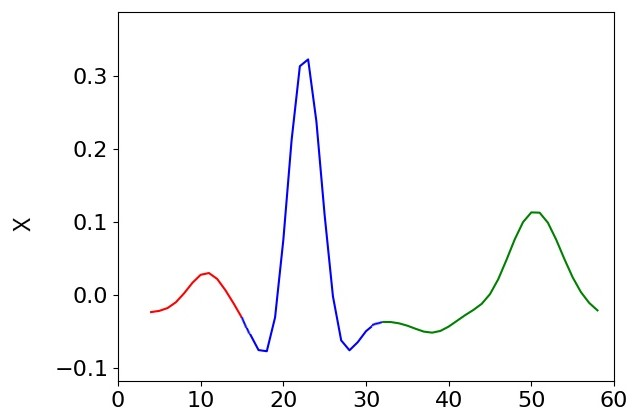
\includegraphics[width=1\textwidth]{images/lead_x.png}
            \captionsetup{justification=centering}
            \caption{}
            \label{fig:lead_x}
        \end{subfigure}
        \begin{subfigure}{\textwidth}
            \centering
            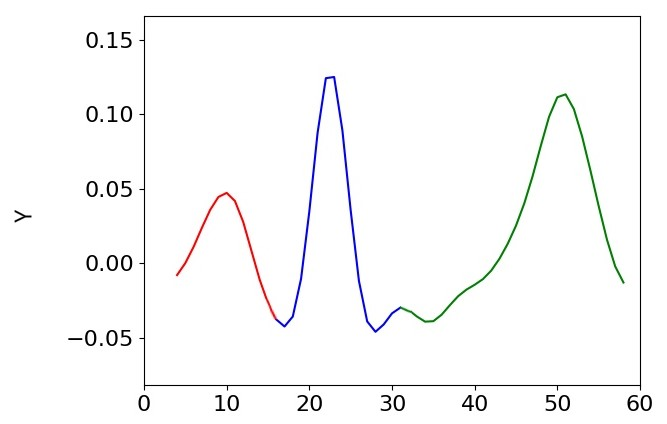
\includegraphics[width=1\textwidth]{images/lead_y.png}
            \captionsetup{justification=centering}
            \caption{}
            \label{fig:lead_y}
        \end{subfigure}
        \begin{subfigure}{\textwidth}
            \centering
            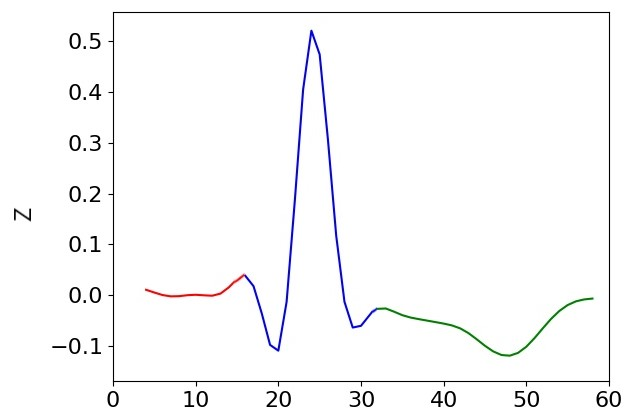
\includegraphics[width=1\textwidth]{images/lead_z.png}
            \caption{}
            \label{fig:lead_z}
        \end{subfigure}
    \end{subfigure}
    \begin{subfigure}{0.55\textwidth}
        \centering
        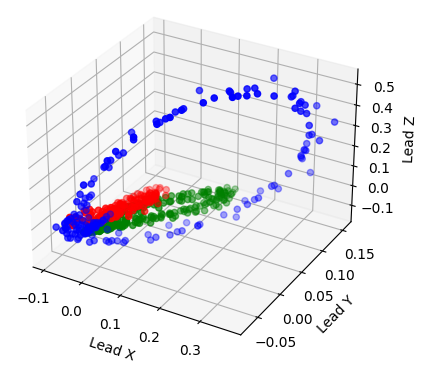
\includegraphics[width=1\linewidth]{images/frank_3d.png}
        \captionsetup{justification=centering}
        \caption{}
        \label{fig:frank_3d}
    \end{subfigure}
    \captionsetup{justification=centering}
    \caption{Figures \ref{fig:lead_x}, \ref{fig:lead_y}, and \ref{fig:lead_z} respectively represent the X, Y, and Z leads of a single beat of an ECG, while Figure \ref{fig:frank_3d} represents a three-dimensional view of a single ECG with respect to the X, Y, and Z axes.}
    \label{fig:ecg}
\end{figure}

\section{Deep Learning}
\label{sec:deep}

The field of ECG analysis has undergone a significant transformation thanks to the application of deep learning techniques. These advanced artificial intelligence (AI) methodologies have shown great promise in improving the accuracy and efficiency of diagnosing and classifying cardiac conditions. Over the years, researchers have developed and refined a variety of neural architectures, including convolutional neural networks (CNNs) and recurrent neural networks (RNNs), to automatically and efficiently analyze ECGs.

In particular, convolutional neural networks have proven to be well-suited for cardiac arrhythmia classification due to their ability to automatically learn relevant features from data. They excel at capturing complex patterns and identifying signals of interest, enabling physicians to obtain more accurate and timely results in diagnosing heart diseases. On the other hand, recurrent neural networks are capable of modeling temporal dependencies present in ECGs and are used for tasks such as anomaly detection and prediction of cardiac events.

A key aspect in applying deep learning to ECG analysis is the availability of large and high-quality training datasets. These datasets contain thousands of expert-annotated ECG recordings, allowing neural networks to learn from past cases and make accurate predictions on new data. However, collecting and annotating these datasets still pose a significant challenge, requiring considerable human effort and collaboration between physicians and researchers.

The application of deep learning to ECG analysis offers many opportunities but also presents several challenges. The network's robustness to signal variations, interpretability of the network's decisions, and the need for customization to adapt to different clinical contexts are some of the issues to consider. Furthermore, integrating deep learning technologies into clinical practice requires careful evaluation of risks, safety, and ethical considerations.

One of the main challenges in applying deep learning to ECGs is the scarcity of labeled data available. Accurate data labeling requires the expertise of experienced physicians to identify and annotate cardiac anomalies. This process can be labor-intensive and time-consuming. Consequently, there is often a limited amount of labeled data available, which can affect the neural networks' ability to generalize and achieve accurate results. Since ECGs can vary significantly among patients, even with the same cardiac condition, variability may be due to numerous factors such as age, sex, electrode placement, and individual physiological conditions. This variability poses a challenge for neural networks as they need to recognize and adapt to these individual differences to achieve accurate and reliable outcomes.

However, before applying AI analysis algorithms and models, adequate preprocessing of ECGs is necessary. Preprocessing plays a crucial role in enhancing signal quality by eliminating unwanted noise and preparing data for proper analysis. ECGs are often affected by noise such as electrical interference or muscle movements, which can compromise the accuracy of subsequent analyses. ECG preprocessing involves applying filtering techniques to remove unwanted noise and isolate the pure cardiac signal. This yields a cleaner representation of the signal and facilitates the identification of significant patterns and anomalies. For instance, baseline artifact is a common phenomenon in ECGs caused by patient movements or electrode positions, and such noise can interfere with neural networks' accurate signal interpretation. Through these preprocessing techniques, it is possible to reduce baseline artifact and obtain a more stable and accurate signal~\cite{use}.

Despite these challenges, the results obtained so far are highly promising: the combination of medical expertise and deep learning knowledge is opening new avenues in ECG analysis, enabling more accurate, timely, and personalized diagnoses for patients. The use of deep learning in ECG analysis is a rapidly evolving research field and will continue to make significant contributions to clinical cardiology practice.

In conclusion, the potential of deep learning in ECG analysis is vast: the integration of advanced AI models with clinical insights offers unprecedented opportunities to enhance the diagnosis, prognosis, and management of cardiac diseases. Ongoing research and collaboration between physicians and researchers will be crucial to fully harnessing the potential of these technologies and delivering tangible benefits to patients with cardiac conditions.

\section{Research Objective}
\label{sec:objective}

The objective of this research was to reconstruct, starting from an electrocardiogram (ECG), the signal that would ideally precede and follow it over time. This required preliminary analysis of the ECGs under examination to subsequently define and train a convolutional neural network (CNN) using deep learning techniques, aimed at predicting the evolution of the ECG itself.

Since clinics still heavily use paper-based ECGs, which span a duration of ten seconds—where the first five seconds display the first 6 leads of the ECG and the remaining five seconds display the remaining 6 leads—the goal was to reconstruct the leads that are not observed: specifically, the first 6 in the latter five seconds and the second 6 in the first five seconds, based on the initial available information.

The entire process was conducted using the Python programming language.

\chapter{Materials and Methods}
\label{chap:materials}

\section{Dataset}
\label{sec:dataset}

The dataset used for this research is \textit{PTB-XL}, an extensive collection of ECGs developed in Germany, containing high-resolution signal recordings from patients with a wide range of cardiac conditions. This dataset was created for research purposes and provides a comprehensive array of signals, including both 12-lead and 15-lead data. It includes ECGs from both healthy patients and those with cardiac abnormalities, enabling users to explore and analyze various clinical cases. As such, it has become a valuable resource for experts in deep learning and AI in the field of cardiology, offering a large dataset for training and evaluating neural networks for cardiac disease diagnosis and classification~\cite{datasetdistro}.

\textit{PTB-XL} comprises a large dataset of 21,799 12-lead ECGs from 18,869 patients, each lasting 10 seconds. The raw waveform data has been annotated by one or two cardiologists who potentially assigned multiple ECG statements to each record. All 71 different ECG statements conform to the \textit{SCP-ECG} standard and include diagnostic, shape, and rhythm statements. Furthermore, the dataset includes detailed metadata on demographics, infarction characteristics, diagnostic statement likelihoods, and reported properties. The waveform data was collected over nearly seven years, from October 1989 to June 1996. During its release in 2019, the existing dataset was optimized with a focus on usability and accessibility for the deep learning community, with waveforms and metadata converted into data formats easily processed by standard software~\cite{dataset}~\cite{datasetref}.

Additionally, each ECG in the dataset exists in two versions: one sampled at \texttt{100 Hz} and another at \texttt{500 Hz}. For this research, ECGs sampled at \texttt{100 Hz} were selected.

\section{Signal Selection and Filtering}
\label{sec:filtering}

Since the considered dataset includes ECGs from patients with cardiac abnormalities, it was initially necessary to filter the signals to include only ECGs from healthy patients.

From Table \ref{tab:dataset} below, the number of ECGs used in the research can be observed:

\begin{table}[H]
    \centering
    \begin{tabular}{|>{\centering\arraybackslash}m{3.5cm}|c|c|}
	\hline Record Count & Superclass & Brief Description \\ \hline
	9514 & NORM & Normal ECGs \\
	5469 & MI & Myocardial Infarction \\
	5235 & STTC & ST/T Wave Abnormality \\
    4898 & CD & Conduction Disorder \\
    2649 & HYP & Hypertrophy \\ \hline
    \end{tabular}
    \captionsetup{justification=centering}
    \caption{Distribution of aggregated diagnostic statements into superclasses. Note: The sum of statements exceeds the number of records in the dataset due to possible multiple labels per record.}
    \label{tab:dataset}
\end{table}

The filtering was performed using two cutoff frequencies, \texttt{0.5 Hz} and \texttt{15 Hz}, used to calculate the low-pass and high-pass filter frequencies. These were then employed in the implemented Butterworth filter to maintain a flat frequency response in the passband. Subsequently, each ECG underwent Gustafson filtering, aimed at improving ECG quality by reducing noise and other unwanted interferences, especially at the signal edges. The technique used is known as \texttt{filtfilt} or zero-phase filtering, where a signal is processed to attenuate unwanted components while preserving the time delay between different signal frequencies. In other words, zero-phase filtering is a technique that removes the delay in the filtered signal, allowing for a more accurate representation of the original signal. This is particularly important in cases where preserving the delay between signal frequencies is crucial for analysis, as in this research context.

From Figure \ref{fig:filtering} below, the differences between the original signal and the filtered signal can be observed:

\begin{figure}[H]
    \centering
    \includegraphics[width=1\textwidth]{images/filtering.png}
    \captionsetup{justification=centering}
    \caption{Differences between the original signal (in blue) and the filtered signal (in red) after applying Gustafson filtering.}
    \label{fig:filtering}
\end{figure}

Finally, the snippet \ref{snippet:filtering} below illustrates the code of the function used to perform the aforementioned operations:

\lstset{language=Python}
\begin{lstlisting}[aboveskip=15pt, belowskip=15pt, basicstyle=\fontsize{8}{10}\selectfont, keywordstyle=\color{blue}, breaklines=true, label=snippet:filtering]
def FilterSignals(signal, fs = 100, do_plot = False):
    f_low = 0.5
    f_high = 15
    order = 3
    nyquist_freq = 0.5 * fs
    lowcut = f_low / nyquist_freq
    highcut = f_high / nyquist_freq
    b, a = butter(order, [lowcut, highcut], btype = 'band')
    filtered_signal = filtfilt(b, a, signal, axis = 1, method = 'gust')
    if do_plot:
        plt.figure(figsize = (10, 4))
        plt.plot(signal, 'b-', label = 'Original ecg')
        plt.plot(filtered_signal, 'r-', label = 'Filtered ecg')
        plt.xlabel('Time [s]')
        plt.ylabel('Amplitude [mV]')
        plt.legend()
        plt.grid(True)
        plt.show()
    return filtered_signal
\end{lstlisting}

\section{Inverse Dower Transformation}
\label{sec:matrice}

The inverse Dower transformation refers to a process used in ECG analysis to obtain a spatial representation of cardiac signals. During the Dower transformation, ECG signals are projected onto a set of orthogonal axes defined as Frank leads, which represent the directions of electrical flow passing through the heart. The inverse Dower transformation is the process that allows retrieving the signals back from their spatial representation according to the Frank leads.

Through this inverse transformation, it is possible to obtain a representation of the signals in the time and amplitude domain, returning to the visualization of the signals as temporal plots of voltage variations over time~\cite{dower}.

The table \ref{tab:dower} below indicates the weights obtained from the inverse Dower matrix~\cite{dowerecg}:

\begin{table}[H]
    \centering
    \begin{tabular}{|*{4}{>{\centering\arraybackslash}m{2.5cm}|}}
    \hline 
    \textit{Lead} & X & Y & Z \\
    \hline
    V1 & -0.17245 & 0.057224 & -0.22891 \\
    V2 & -0.07377 & -0.018954 & -0.31001 \\
    V3 & 0.12222 & -0.10637 & -0.24588 \\
    V4 & 0.23103 & -0.021986 & -0.063351 \\
    V5 & 0.23931 & 0.040947 & 0.054782 \\
    V6 & 0.19358 & 0.048257 & 0.10849 \\
    I & 0.15608 & -0.22739 & 0.021654 \\ 
    II & -0.0099152 & 0.88653 & 0.10207 \\ \hline
    \end{tabular}
    \captionsetup{justification=centering}
    \caption{Weights obtained from the inverse Dower matrix, in this case transposed compared to the original matrix.}
    \label{tab:dower}
\end{table}

In figure \ref{fig:frank_2d} below, you can observe the two-dimensional representation of the three X, Y, and Z leads of a single ECG:

\begin{figure}[H]
    \centering
    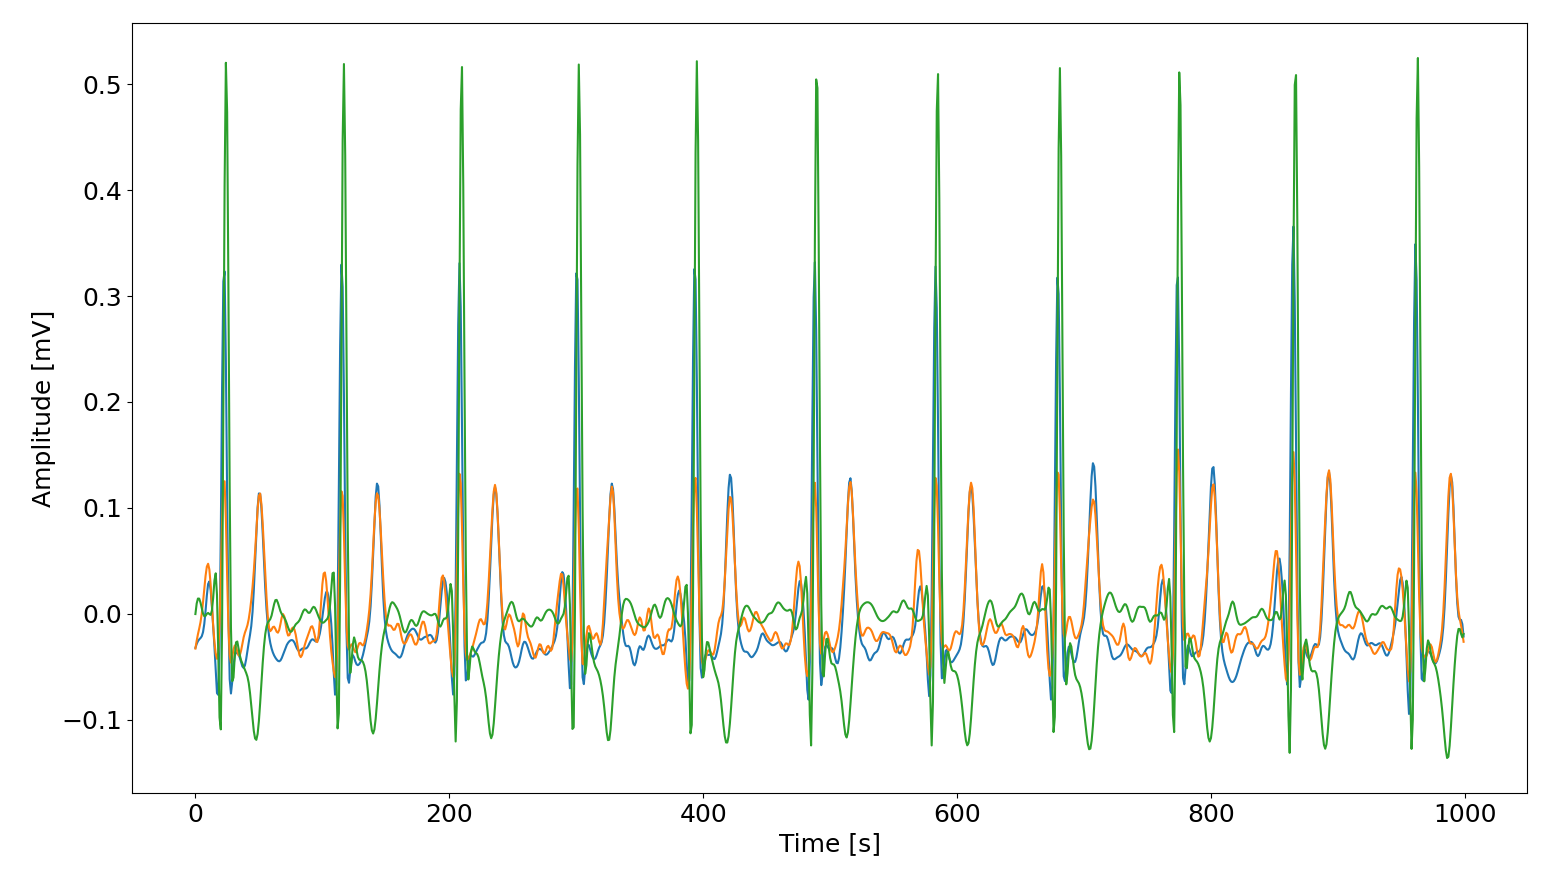
\includegraphics[width=1\textwidth]{images/frank_2d.png}
    \captionsetup{justification=centering}
    \caption{Two-dimensional representation of the three X, Y, and Z leads of a single ECG.}
    \label{fig:frank_2d}
\end{figure}

Finally, the snippet \ref{snippet:dower} below illustrates the code of the function used for the application of the inverse Dower transformation:

\lstset{language=Python}
\begin{lstlisting}[aboveskip=15pt, belowskip=15pt, basicstyle=\fontsize{8}{10}\selectfont, keywordstyle=\color{blue}, breaklines=true, label=snippet:dower]
def ApplyInverseMatrix(signal, do_plot = False):
    matrix = pd.read_csv('inverse_dower.csv', header = None)
    weights = torch.tensor(matrix.values, dtype = torch.float64)
    ponderate_ecg = torch.matmul(weights, signal)
    if do_plot:
        plt.figure(figsize = (10, 6))
        plt.plot(ponderate_ecg.T)
        plt.xlabel('Time [s]')
        plt.ylabel('Amplitude [mV]')
        plt.title('ECG Leads: X, Y, Z')
        plt.show()
    return ponderate_ecg
\end{lstlisting}

\section{Entropy}
\label{sec:entropia}

Entropy of a matrix refers to a measure of its complexity or uncertainty. In general, the entropy of a uniform distribution is the maximum possible entropy, while the entropy of a constant distribution is always zero. Therefore, higher entropy indicates greater diversity among the data.

The objective was to reconstruct the six signals [$ V_{1}, V_{2}, V_{3}, V_{4}, V_{5}, V_{6} $] from the other six signals [$ I, II, III, aV_{R}, aV_{L}, aV_{F} $]. The former primarily lie on the horizontal plane while the latter on the frontal plane. This means that it wouldn't actually be possible to determine each of the former signals [$ V_{1}, V_{2}, V_{3}, V_{4}, V_{5}, V_{6} $] from the latter signals [$ I, II, III, aV_{R}, aV_{L}, aV_{F} $], because Equation (\ref{eq:lead}) does not hold:

\begin{equation}
    V_{n} = f_{n}(I, II, III, aV_{R}, aV_{L}, aV_{F})
    \label{eq:lead}
\end{equation}

However, this actually depends on how probable $ V_{n} $ is given the values of the other leads. For instance, if $ V_{n} $ were always equal to \texttt{1 mV}, then it would be possible to define the function $ f_{n} $ as $ f_{n} = 1 $. In such a case, the entropy would be minimal because $ V_{1} $ would consistently point to \texttt{1 mV} on the horizontal plane, resulting in a histogram spike.

With that said, it is possible to project the Frank leads X, Y, and Z onto a bidimensional plane in order to calculate their histograms. Using the histogram as an estimate of the probability density function, it is then possible to calculate the entropy to understand how predictable it is.

The immediate next step was to calculate the two-dimensional distributions related to each histogram, in turn, related to each ECG.

Thanks to each of these distributions, it was then possible to calculate their total sum to represent a total distribution over time. This distribution, represented on the X, Y, and Z axes, identifies the cells of the distributions in which the points of each ECG are located, and is crucial for calculating entropy.

In figure \ref{fig:histogram_single_beat} below, you can see the bidimensional representation of the histogram of a single beat of a certain ECG:

\begin{figure}[H]
    \centering
    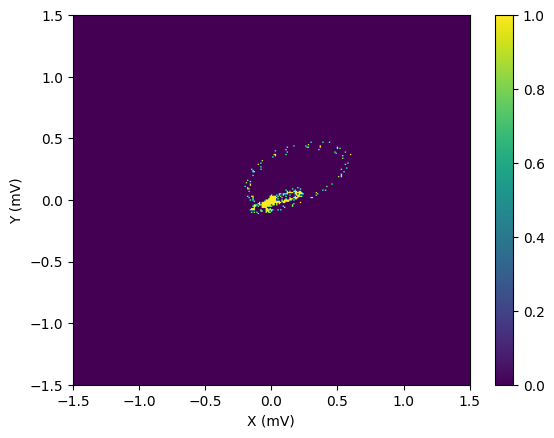
\includegraphics[width=0.65\textwidth]{images/histogram_single_beat.png}
    \captionsetup{justification=centering}
    \caption{Bidimensional representation of the histogram of the distribution of a single beat of an ECG.}
    \label{fig:histogram_single_beat}
\end{figure}

Figure \ref{fig:each_beat_all_ecg} below instead illustrates the representation of the matrix containing the sum of the two-dimensional distributions related to each beat of all ECGs of all considered patients:

\begin{figure}[H]
    \centering
    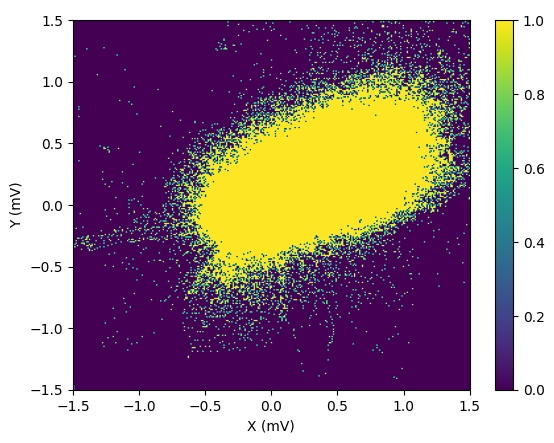
\includegraphics[width=0.65\textwidth]{images/each_beat_all_ecg.png}
    \captionsetup{justification=centering}
    \caption{Representation of the matrix containing the sum of the two-dimensional distributions related to each beat of all ECGs.}
    \label{fig:each_beat_all_ecg}
\end{figure}

Entropy can be calculated using different formulas depending on the specific context. For instance, for a probability matrix, entropy can be calculated using a generalization of Shannon's entropy formula (\ref{eq:shannon}), as shown below:

\begin{equation}
    H = - \sum_{x,y} p(x,y) \log_2(p(x,y))
    \label{eq:shannon}
\end{equation}

The formula represents the joint Shannon entropy $ H $ of two discrete variables $ x $ and $ y $, which is a generalization to two or more variables of Shannon's formula. Specifically, the symbol $ \sum_{x,y} $ indicates a summation over all possible combinations of values of $ x $ and $ y $, $ p(x,y) $ represents the joint probability that variables $ x $ and $ y $ assume certain values simultaneously, while $ \log_2(p(x,y)) $ is the binary logarithm of the joint probability of $ x $ and $ y $, i.e., the probability that both variables assume certain values simultaneously.

The snippet \ref{snippet:entropia} below shows the code of the function used for calculating entropy, based on the formula illustrated above:

\lstset{language=Python}
\begin{lstlisting}[aboveskip=15pt, belowskip=15pt, basicstyle=\fontsize{8}{10}\selectfont, keywordstyle=\color{blue}, breaklines=true, label=snippet:entropia]
def CalculateEntropy(hists_matrix):
    probabilities = hists_matrix / np.sum(hists_matrix)
    entropy = -np.sum(probabilities * np.log2(probabilities + np.finfo(float).eps))
    max_entropy = np.log2(hists_matrix.shape[0] * hists_matrix.shape[1])
    print(entropy / max_entropy)
\end{lstlisting}

Finally, another formula (\ref{eq:entropia}) was used during the research, shown below, which computes a numerical index called \textit{predictability index} ranging between \texttt{0} and \texttt{1}. Here, \texttt{0} indicates a uniform distribution where $ H = H_{u} $, with $ H_{u} $ being the entropy of a uniform distribution, thus it is \textit{completely unpredictable}. Conversely, \texttt{1} indicates a non-uniform distribution where $ H = 0 $ thus it is \textit{completely predictable} or \textit{constant}:

\begin{equation}
    h = \frac{H_{u} - H}{H_{u}}
    \label{eq:entropia}
\end{equation}

\section{Problem Modeling}
\label{sec:modellazione}

The model that has been constructed is based on a CNN, chosen due to the highly promising results observed in other studies and its efficiency in terms of computational resources, making it suitable for training on large datasets, as required in this research context~\cite{ribeiro}~\cite{hannun}.

The model, irrespective of the complexity of various CNN architectures implemented, receives 12 leads as input divided into two blocks of 6 leads each, with each block representing a duration of five seconds. Thus, the initial information available is dual: the first set of 6 leads in the first five seconds and the second set of 6 leads in the subsequent five seconds. The output of the model, however, consists of the leads that are not directly observed: the first 6 leads in the second five seconds and the second 6 leads in the first five seconds.

The constructed model can be summarized mathematically with equation (\ref{eq:modello}), where $ x $ denotes the ECG signals constituting the input, and $ y $ denotes the ECG signals constituting the output:

\begin{equation}
    y = f(x)
    \label{eq:modello}
\end{equation}

However, the problem at hand is not trivial because each ECG is a complex and multi-dimensional signal, composed of various components including the P-wave, Q-wave, R-wave, S-wave, and T-wave. Each component has its own shape and duration, and their interrelationship is crucial for the interpretation of each ECG.

\section{Convolutional neural network}
\label{sec:network}

\subsection{Formal description}
\label{subsec:descrizione}

During the research, numerous CNNs were implemented and tested, each significantly different from the others, aimed at obtaining diverse results regarding the reconstruction of ECG signals.

Each CNN was implemented as a class, defined by two functions, \texttt{init()} and \texttt{forward()}. These functions are respectively used to instantiate the class representing the CNN and to define the data flow through the network, where input data propagate through various layers to generate the final output.

During initialization, the various layers of the CNN are defined, including convolutional layers, pooling layers, fully connected layers, and activation functions. Within the \texttt{init()} function, fundamental network parameters are set, such as convolutional filter sizes, number of feature maps, pooling function sizes, input and output dimensions, and many other parameters that influence its performance. Additionally, this phase may involve creating other variables necessary for managing data and layer weights.

In the \texttt{forward()} function, convolution, pooling, and activation operations are performed, allowing the network to learn complex representations from the input data. During the execution of \texttt{forward()}, input data pass through the layers, and weights are applied to the feature maps to produce the final output. Each layer has its own weights and biases that are updated during the network training phase, enabling the CNN to learn how to recognize relevant patterns and features in the data. Importantly, the \texttt{forward()} function is subsequently executed during the evaluation phase of the network when it is used to make predictions on new input data. This forward propagation process allows the CNN to produce the desired output based on the weights acquired during the training phase.

\subsection{First CNN}
\label{subsec:first_cnn}

The snippet \ref{snippet:first_cnn} below represents the code of one of the first CNNs implemented and tested, which, however, did not yield the expected results initially:

\lstset{language=Python}
\begin{lstlisting}[aboveskip=15pt, belowskip=15pt, basicstyle=\fontsize{8}{10}\selectfont, keywordstyle=\color{blue}, breaklines=true, label=snippet:first_cnn]
class ConvNet(nn.Module):
    def __init__(self, input_shape):
        super(ConvNet, self).__init__()
        self.input_shape = input_shape
        self.conv1 = nn.Conv1d(in_channels = self.input_shape[0], out_channels = 32, kernel_size = 8)
        self.conv2 = nn.Conv1d(in_channels = 32, out_channels = 64, kernel_size = 8)
        self.maxpool = nn.MaxPool1d(kernel_size = 2)
        self.flatten = nn.Flatten()
        self.fc1 = nn.Linear(7616, 128)
        self.relu = nn.ReLU()
        self.output = nn.Linear(128, self.input_shape[0] * self.input_shape[1])
    def forward(self, x):
        with open(f'{OUTPUTS_DIRECTORY}/model_settings.txt', 'w') as file:
            file.write(f'conv_kernel_size = {self.conv1.kernel_size[0]}, maxpool_kernel_size = {self.maxpool.kernel_size}')
        x = x.to(device)
        x = x.type(torch.DoubleTensor)
        x = x.to(device)
        x = self.conv1(x)
        x = self.relu(x)
        x = self.maxpool(x)
        x = self.conv2(x)
        x = self.relu(x)
        x = self.maxpool(x)
        x = self.relu(x)
        x = self.flatten(x)
        x = self.fc1(x)
        x = self.relu(x)
        x = self.output(x)
        x = torch.reshape(x, (-1, self.input_shape[0], self.input_shape[1]))
        return x
\end{lstlisting}

The figure \ref{fig:first_cnn_layers} below depicts, in the form of a flowchart, the layers constituting the code snippet \ref{snippet:first_cnn} of the first CNN, provided immediately above.

\begin{figure}[H]
    \centering
    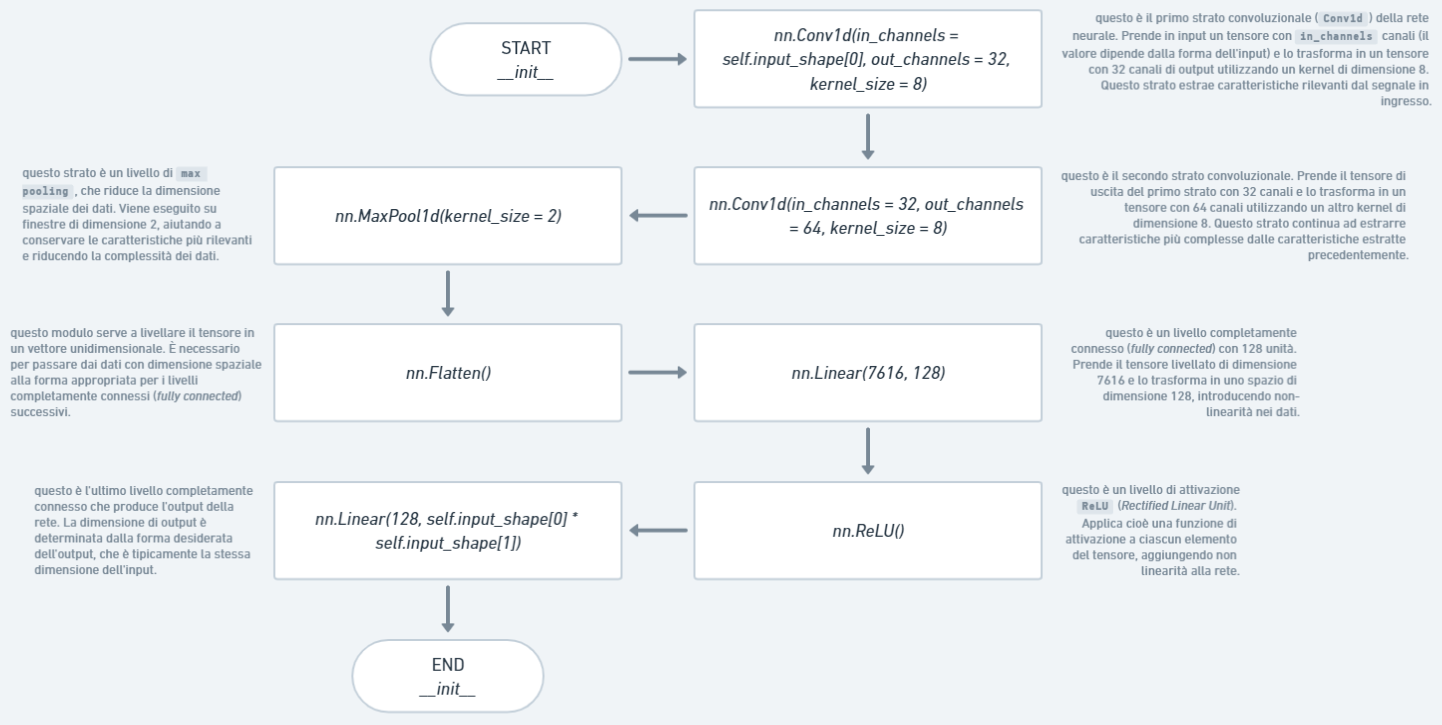
\includegraphics[width=1\textwidth]{images/first_cnn_layers.png}
    \captionsetup{justification=centering}
        \caption{Flowchart representation of the layers in the code snippet.}
    \label{fig:first_cnn_layers}
\end{figure}

This first CNN includes only a \textit{ConvNet}, whose code consists of a set of convolutional layers that are repeated several times in the \texttt{forward()} function, acting on the input parameters.

\subsection{Second CNN}
\label{subsec:second_cnn}

The snippet \ref{snippet:second_cnn} below represents the code of another CNN defined as "intermediate" in terms of complexity among all the CNNs used in the research. However, like the first CNN, it also did not yield the expected results:

\lstset{language=Python}
\begin{lstlisting}[aboveskip=15pt, belowskip=15pt, basicstyle=\fontsize{8}{10}\selectfont, keywordstyle=\color{blue}, breaklines=true, label=snippet:second_cnn]
class ResidualBlock(nn.Module):
    def __init__(self, in_channels, out_channels, kernel_size):
        super(ResidualBlock, self).__init__()
        self.conv = nn.Conv1d(in_channels, out_channels, kernel_size, padding = 'same')
        self.relu = nn.ReLU()
    def forward(self, x):
        x = x.to(device)
        x = x.type(torch.DoubleTensor)
        out = self.conv(x)
        out = self.relu(out)
        return x + out
class ConvNet(nn.Module):
    def __init__(self, input_shape):
        super(ConvNet, self).__init__()
        self.input_shape = input_shape
        self.conv1 = ResidualBlock(in_channels = self.input_shape[0], out_channels = self.input_shape[0], kernel_size = 32)
        self.conv2 = nn.Conv1d(in_channels = self.input_shape[0], out_channels = 32, kernel_size = 16)
        self.conv3 = ResidualBlock(in_channels = 32, out_channels = 32, kernel_size = 16)
        self.conv4 = nn.Conv1d(in_channels = 32, out_channels = 16, kernel_size = 5)
        self.conv5 = ResidualBlock(in_channels = 16, out_channels = 16, kernel_size = 5)
        self.conv6 = nn.Conv1d(in_channels = 16, out_channels = 128, kernel_size = 3)
        self.maxpool = nn.MaxPool1d(kernel_size = 2)
        self.flatten = nn.Flatten()
        self.fc1 = nn.Linear(6656, 128)
        self.relu = nn.ReLU()
        self.output = nn.Linear(128, self.input_shape[0] * self.input_shape[1])
    def forward(self, x):
        x = self.conv1(x)
        x = self.relu(x)
        x = self.maxpool(x)
        x = self.conv2(x)
        x = self.relu(x)
        x = self.maxpool(x)
        x = self.conv3(x)
        x = self.relu(x)
        x = self.maxpool(x)
        x = self.conv4(x)
        x = self.relu(x)
        x = self.conv5(x)
        x = self.relu(x)
        x = self.conv6(x)
        x = self.flatten(x)
        x = self.fc1(x)
        x = self.relu(x)
        x = self.output(x)
        x = torch.reshape(x, (-1, self.input_shape[0], self.input_shape[1]))
        return x
\end{lstlisting}

Figure \ref{fig:second_cnn_layers} below represents, in the form of a flowchart, the layers that constitute the code \ref{snippet:second_cnn} of the second CNN, reported immediately above:

\begin{figure}[H]
    \centering
    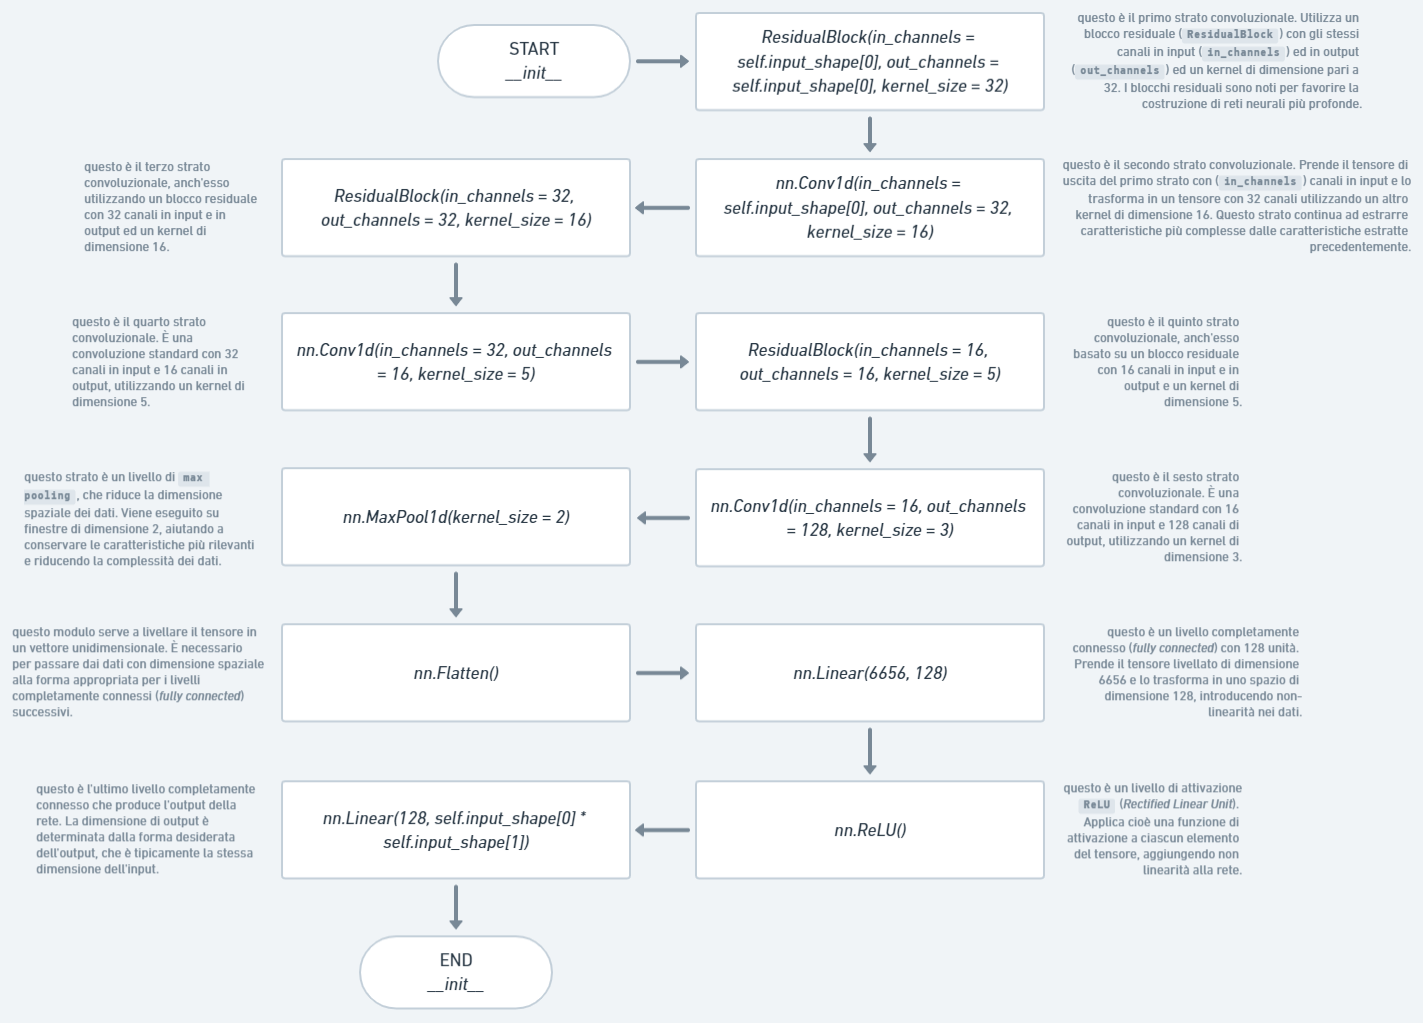
\includegraphics[width=1\textwidth]{images/second_cnn_layers.png}
    \captionsetup{justification=centering}
    \caption{Flowchart representation of the layers in the code snippet.}
    \label{fig:second_cnn_layers}
\end{figure}

This "intermediate" CNN includes only a \textit{ConvNet}, whose code consists of a set of convolutional layers combined with an external component called a \textit{Residual Block}. This block is introduced to address the issue of performance degradation as networks become deeper, and is implemented as a class representing a standalone module of the CNN designed to learn more refined features from the data. The underlying idea is to allow data to bypass one or more convolutional layers, so that each bypassed flow is then added to the outputs of subsequent convolutional layers. This addition of the bypassed flow enhances backward gradient propagation during training, facilitating the learning of more effective representations.
By implementing the \textit{Residual Block} as a class, a reusable module has been created that can easily be incorporated into various CNN architectures, simplifying the code structure and making the entire CNN more modular. This approach facilitates further experiments and modifications.

\subsection{Third CNN}
\label{subsec:third_cnn}

Finally, snippet \ref{snippet:third_cnn} below represents the code of the last CNN, in chronological order of testing, implemented and evaluated:

\lstset{language=Python}
\begin{lstlisting}[aboveskip=15pt, belowskip=15pt, basicstyle=\fontsize{8}{10}\selectfont, keywordstyle=\color{blue}, breaklines=true, label=snippet:third_cnn]
class ResidualBlock(nn.Module):
    def __init__(self, in_channels, out_channels, kernel_size):
        super(ResidualBlock, self).__init__()
        self.conv = nn.Conv1d(in_channels, out_channels, kernel_size, padding = 'same')
        self.relu = nn.ReLU()
    def forward(self, x):
        out = self.conv(x)
        out = self.relu(out)
        return x + out
class ConvNet(nn.Module):
    def __init__(self, input_shape):
        super(ConvNet, self).__init__()
        self.input_shape = input_shape
        self.conv1 = ResidualBlock(in_channels = self.input_shape[0], out_channels = self.input_shape[0], kernel_size = 5)
        self.conv2 = nn.Conv1d(in_channels = self.input_shape[0], out_channels = 32, kernel_size = 5)
        self.conv3 = ResidualBlock(in_channels = 32, out_channels = 32, kernel_size = 5)
        self.conv4 = nn.Conv1d(in_channels = 32, out_channels = 64, kernel_size = 5)
        self.conv5 = ResidualBlock(in_channels = 64, out_channels = 64, kernel_size = 5)
        self.conv6 = nn.Conv1d(in_channels = 64, out_channels = 128, kernel_size = 5)
        self.maxpool = nn.MaxPool1d(kernel_size = 2)
        self.flatten = nn.Flatten()
        self.fc1 = nn.Linear(6784, 128)
        self.relu = nn.ReLU()
        self.output = nn.Linear(128, self.input_shape[0] * self.input_shape[1])
    def forward(self, x):
        with open(f'{OUTPUTS_DIRECTORY}/model_settings.txt', 'w') as file:
            file.write(f'conv_kernel_size = 5, maxpool_kernel_size = 2')
        x = self.conv1(x)
        x = self.relu(x)
        x = self.maxpool(x)
        x = self.conv2(x)
        x = self.relu(x)
        x = self.maxpool(x)
        x = self.conv3(x)
        x = self.relu(x)
        x = self.maxpool(x)
        x = self.conv4(x)
        x = self.relu(x)
        x = self.conv5(x)
        x = self.relu(x)
        x = self.conv6(x)
        x = self.flatten(x)
        x = self.fc1(x)
        x = self.relu(x)
        x = self.output(x)
        x = torch.reshape(x, (-1, self.input_shape[0], self.input_shape[1]))
        return x

class CustomLayer(torch.nn.Module):
    def __init__(self, d = 25, r = 45):
        super(CustomLayer, self).__init__()
        self.d = d
        self.r = r
        self.b1 = np.array([0.0008, 0.0026, 0.0055, 0.0092, 0.0119, 0.0100, -0.0000, -0.0194, -0.0449, -0.0685, -0.0794, -0.0688, -0.0340, 0.0189, 0.0758, 0.1195, 0.1359, 0.1195, 0.0758, 0.0189, -0.0340, -0.0688, -0.0794, -0.0685, -0.0449, -0.0194, -0.0000, 0.0100, 0.0119, 0.0092, 0.0055, 0.0026, 0.0008])
        self.filter_order = len(self.b1)
        self.conv1d_1 = nn.Conv1d(in_channels = 6, out_channels = 1, kernel_size = self.filter_order, padding = 'same', bias = False)
        p = self.conv1d_1.state_dict()
        for i in range(len(self.b1)):
            for f in range(6):
                p['weight'][0][f][i] = self.b1[i]
        self.mv_avg_order = 10
        self.b2 = np.array([1.0/self.mv_avg_order] * self.mv_avg_order)
        self.conv1d_2 = nn.Conv1d(in_channels = 1, out_channels = 1, kernel_size = self.mv_avg_order, padding = 'same', bias = False)
        p = self.conv1d_2.state_dict()
        for i in range(len(self.b2)):
            p['weight'][0][0][i] = self.b2[i]
    def pan_tompkins(self, ecg):        
        pt = self.conv1d_1(ecg)
        pt = torch.diff(pt, dim = 2, append = torch.zeros(pt.shape[0], 1, 1).to(device))
        pt = pt ** 2
        pt = self.conv1d_2(pt)
        B, _, _ = pt.shape
        for b in range(B):
            pt[b, 0, :] = torch.tanh(3.0 * pt[b, 0, :].clone()/torch.max(pt[b, 0, :].clone()))
        return pt
    def avg_beat(self, ecg, pt):
        B, L, N = ecg.shape
        d = self.d
        r = self.r
        t = torch.zeros(B, L, (d + r)).to(device)
        n_beats = pt[0, 0, d : (N - r)].sum()
        for b in range(B):
            for n in range(0, (d + r)):          
                s = ecg[b, :, n : (N - r + n - d)] @ pt[0, 0, d : (N - r)].to(device)
                t[b, :, n] = s
        return t / n_beats
    def spread(self, t, pt):
        B, L, _ = t.shape
        N = pt.shape[2]
        d = self.d
        r = self.r
        y = torch.zeros(B, L, N)
        y = y.to(device)
        for b in range(B):
            for n in range(r, N - d):
                s = t[b, :, :].float() @ torch.flip(pt[0, 0, (n - r) : (n + d)].float(), tuple([0]))
                y[b, :, n].add_(s)
        return y
    def forward(self, x):
        ecg1 = x[:, :6, :]
        ecg2 = x[:, 6:, :]
        pt1 = self.pan_tompkins(ecg1)
        pt2 = self.pan_tompkins(ecg2)
        t1 = self.avg_beat(ecg1, pt1)
        t2 = self.avg_beat(ecg2, pt2)
        y1 = self.spread(t1, pt2)
        y2 = self.spread(t2, pt1)
        return torch.concatenate((y1, y2), dim = 1)
    
class FinalCustomLayer(nn.Module):
    def __init__(self, input_shape):
        super(FinalCustomLayer, self).__init__()
        self.convnet1 = ConvNet(input_shape)
        self.convnet2 = CustomLayer()
    def forward(self, x):
        output1 = self.convnet1(x)
        output2 = self.convnet2(x)
        output = output1 + output2
        return output
\end{lstlisting}

Figure \ref{fig:third_cnn_layers} below represents, in the form of a flowchart, the layers that constitute the code \ref{snippet:third_cnn} of the third and final CNN, reported immediately above:

\begin{figure}[H]
    \centering
    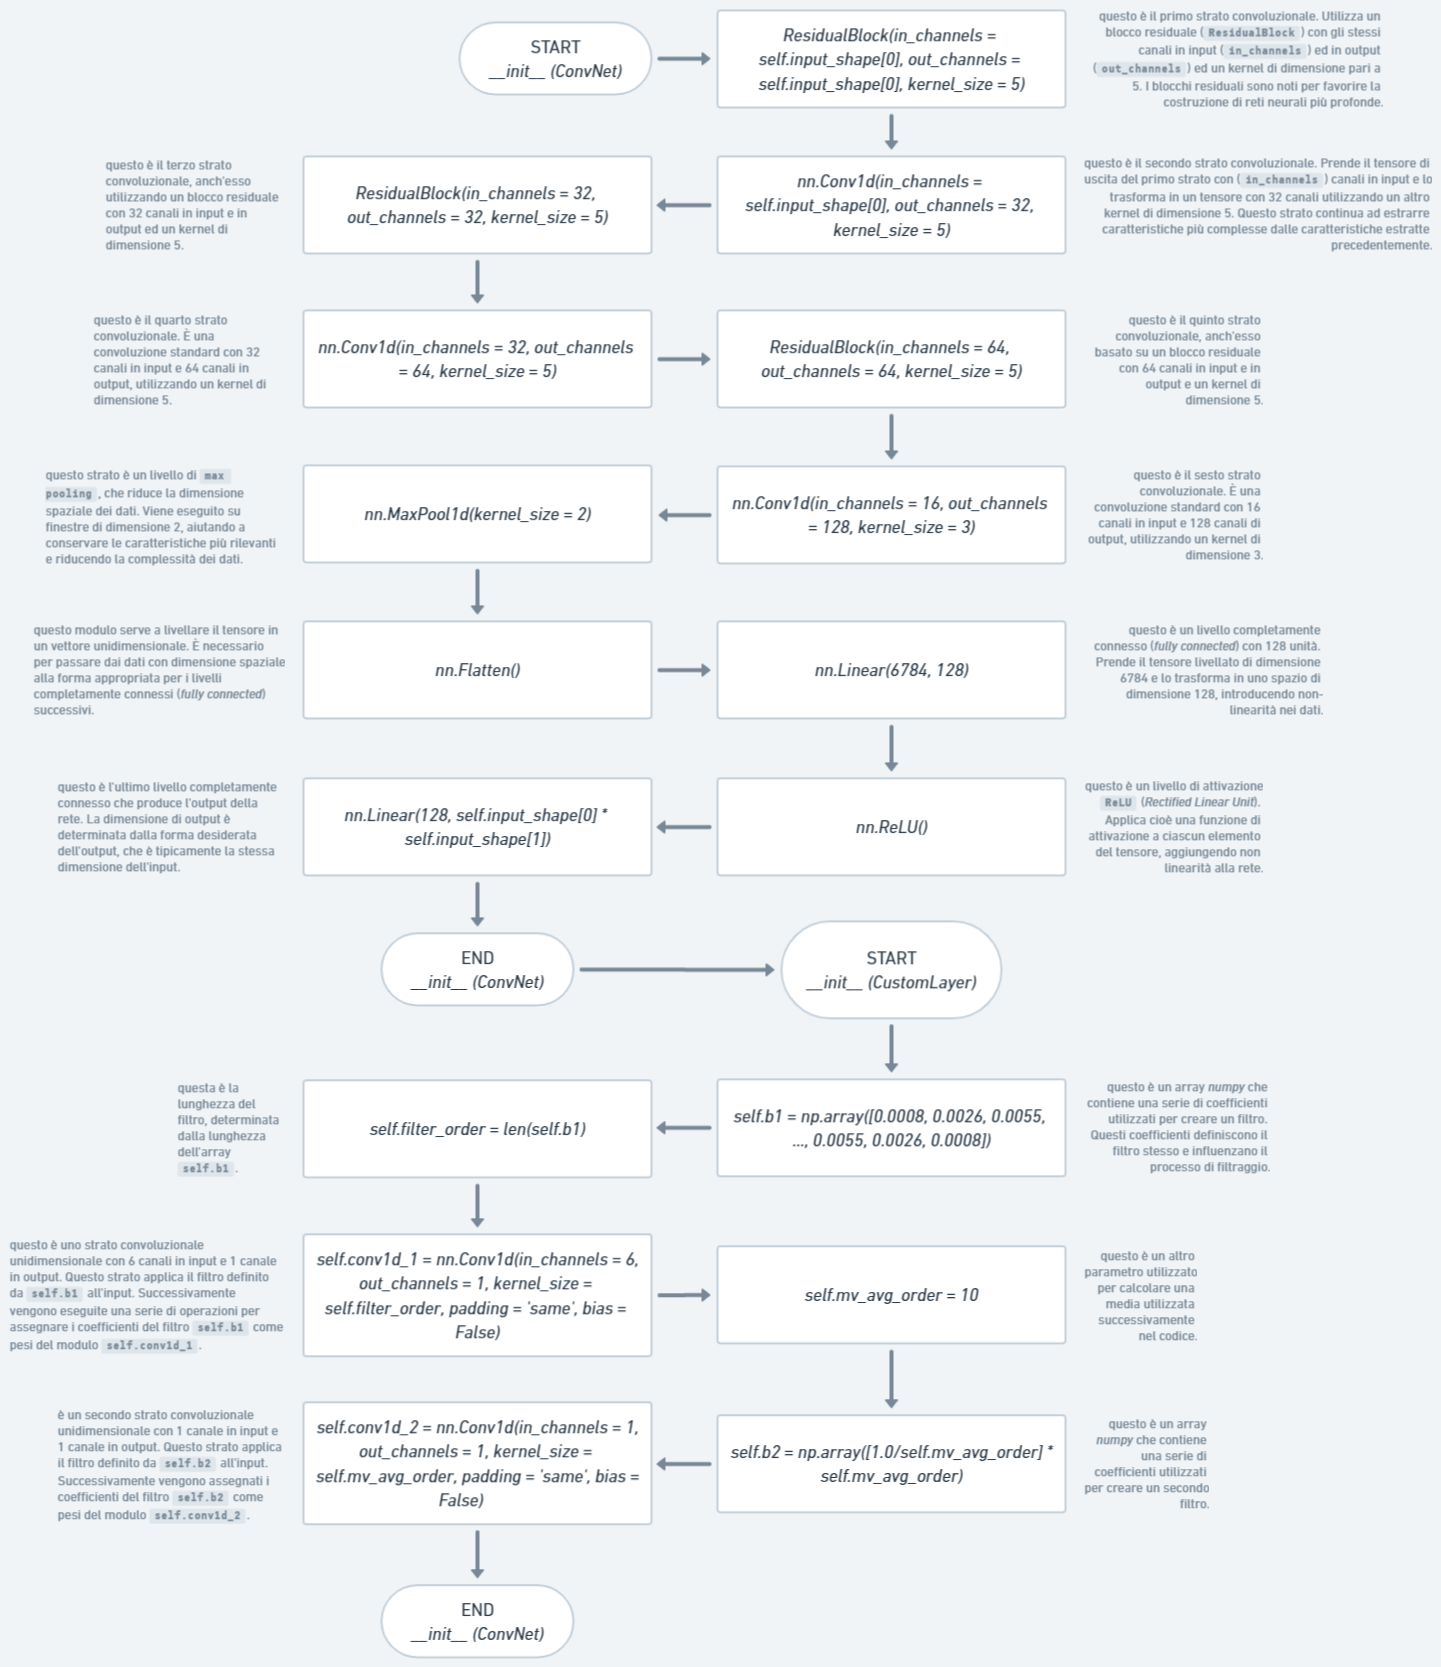
\includegraphics[width=1\textwidth]{images/third_cnn_layers.png}
    \captionsetup{justification=centering}
    \caption{Flowchart representation of the layers in the code snippet.}
    \label{fig:third_cnn_layers}
\end{figure}

This particular CNN implements a Custom Layer called \textit{Final Custom Layer}, which includes a ConvNet and an additional Custom Layer. The ConvNet code is structured exactly like the previous CNN implemented. On the other hand, the Custom Layer's code, in addition to defining the \texttt{init()} and \texttt{forward()} functions, includes three additional function definitions: \texttt{pan\_tompkins()}, \texttt{avg\_beat()}, and \texttt{spread()}. The \texttt{pan\_tompkins()} function was developed to detect peaks of QRS complexes in ECG signals after they have passed through various convolutional layers, acting as a post-processing phase. The \texttt{avg\_beat()} function, on the other hand, computes an average representation of QRS complex peaks within a segment for each ECG. Finally, the \texttt{spread()} function is designed to obtain the average heartbeat and position it correctly in the subsequent six-second predictions. For example, the positions of the heartbeats recorded by leads [$ V_{1}, V_{2}, V_{3}, V_{4}, V_{5}, V_{6} $] are used to estimate the positions of heartbeats in the following six seconds. This estimation is achieved by taking the average heartbeat from leads [$ I, II, III, aV_{R}, aV_{L}, aV_{F} $] and duplicating it for the next six seconds. This duplication is done using cross-correlation between two signals: the first signal representing the average heartbeat and the second signal generated by the \texttt{pan\_tompkins()} function. If the latter is a perfect impulse, the heartbeat would be copied entirely to the position of the impulse.

\section{Training of the CNN}
\label{sec:addestramento}

All CNNs implemented during the research were trained according to the same logic, using two DataLoaders: one for training on the dataset and another for validation.

For all trained CNNs, the same parameters were set and used: \texttt{BATCH\_SIZE} and \texttt{LEARNING\_RATE} were both set to \texttt{16} and \texttt{0.001} respectively. These parameters are crucial for the proper functioning of the entire CNN. \texttt{BATCH\_SIZE} denotes the number of data samples used in each training iteration, while \texttt{LEARNING\_RATE} controls how quickly the CNN adapts to the training data. Additionally, the \texttt{NUM\_EPOCHS} parameter, which indicates the number of training epochs, was set to \texttt{100}. The optimizer used was \texttt{torch.optim.Adam}, an optimization algorithm that combines concepts of stochastic optimizers with adaptive learning rate methods, making it effective for CNN convergence.

In particular, using a larger \texttt{BATCH\_SIZE} can better utilize computational resources and accelerate CNN training, but it also requires more memory. Conversely, a smaller \texttt{BATCH\_SIZE} may be advantageous in terms of efficient memory usage and CNN generalization, but it can take more time for overall training. Similar considerations apply to the \texttt{LEARNING\_RATE}; a higher \texttt{LEARNING\_RATE} leads to faster adaptation but may cause oscillations or suboptimal convergence, while a lower \texttt{LEARNING\_RATE} results in slower adaptation but potentially better convergence to an optimal solution. Finding the right \texttt{LEARNING\_RATE} value is crucial for effective CNN training. A \texttt{LEARNING\_RATE} that is too high may cause instability, while one that is too low may slow down training or cause the CNN to converge to a local minimum instead of the global minimum.

In conclusion, the choice of \texttt{BATCH\_SIZE} and \texttt{LEARNING\_RATE} values depends on the dataset, available computational resources, and specific problem requirements. It is common practice to experiment with different \texttt{BATCH\_SIZE} and \texttt{LEARNING\_RATE} values to find optimal settings for the specific scenario.

Snippet \ref{snippet:addestramento} below represents the code of the function used for training the implemented CNNs:

\lstset{language=Python}
\begin{lstlisting}[aboveskip=15pt, belowskip=15pt, basicstyle=\fontsize{8}{10}\selectfont, keywordstyle=\color{blue}, breaklines=true, label=snippet:addestramento]
list_train_loss = []
list_val_loss =  []
def TrainingModel(model, train_loader, val_loader, loss_fn, optimizer, num_epochs):
    global list_train_loss, list_val_loss
    best_loss = float('inf')
    for epoch in range(num_epochs):
        model.train()
        train_loss = 0.0
        for ecgs, targets in train_loader:
            optimizer.zero_grad()
            outputs = model(ecgs.to(device))
            targets = targets.to(device)
            loss = loss_fn(outputs.float(), targets.float())
            train_loss += loss.item()
            loss.backward()
            optimizer.step()
        avg_train_loss = train_loss / len(train_loader)
        list_train_loss.append(avg_train_loss)
        avg_val_loss = EvaluateModel(model, val_loader, loss_fn)
        list_val_loss.append(avg_val_loss)
        print(f'Epoch {epoch + 1}/{num_epochs}: train_loss = {avg_train_loss: .4f}, val_loss = {avg_val_loss: .4f}')
        with open(f'{OUTPUTS_DIRECTORY}/epochs.txt', 'a') as file:
            file.write(f'Epoch {epoch + 1}/{num_epochs}: train_loss = {avg_train_loss: .4f}, val_loss = {avg_val_loss: .4f}\n')
        if avg_val_loss < best_loss:
            best_loss = avg_val_loss
            torch.save(model.state_dict(), 'best_model.pt')
\end{lstlisting}

\section{Validation of CNN}
\label{sec:validazione}

The validation process was executed by defining a dedicated function to calculate the total number of errors during the evaluation, which is useful for subsequently calculating the average error relative to the total \texttt{BATCH\_SIZE}.

Of crucial importance is the \texttt{LOSS\_FN} parameter passed as input to the function, which is responsible for computing the errors between predictions and targets. It is defined earlier in the code as \texttt{loss = nn.MSELoss()}, typically used in regression problems where the goal is to predict a continuous numerical value. The \texttt{MSE} function, short for Mean Squared Error, computes the squared difference between each element of predictions and targets, and then computes the mean.

In summary, this function evaluates the CNN using the provided validation DataLoader. It iterates through batches of data, passes the data through the CNN to obtain predictions, calculates the error between predictions and targets, and finally computes the average loss across all data batches. This provides an estimate of the CNN's error during the validation phase.

Snippet \ref{snippet:validazione} below represents the code of the function used for validating the implemented CNNs:

\lstset{language=Python}
\begin{lstlisting}[aboveskip=15pt, belowskip=15pt, basicstyle=\fontsize{8}{10}\selectfont, keywordstyle=\color{blue}, breaklines=true, label=snippet:validazione]
def EvaluateModel(model, loader, loss_fn):
    model.eval()
    total_loss = 0.0
    with torch.no_grad():
        for values in loader:
            ecgs = values[0]
            targets = values[1]
            outputs = model(ecgs.to(device))
            targets = targets.to(device)
            loss = loss_fn(outputs.float(), targets.float())
            total_loss += loss.item()
    avg_loss = total_loss / len(loader)
    return avg_loss
\end{lstlisting}

\section{Clustering analysis applied to signals}
\label{sec:clustering}

After determining the poor performance results of the implemented and tested CNNs, an alternative approach was pursued to simplify the training data by using the \textit{K-means} clustering algorithm. \textit{K-means} is widely used in machine learning and data analysis to group similar data points into sets commonly known as clusters. The primary goal of the algorithm is to divide an initial set of data into different clusters, where data points within the same cluster are more similar to each other than to those in other clusters~\cite{cluster}. This approach aims to improve CNN performance by leveraging signal similarity while maintaining a large total dataset crucial for training.

Snippet \ref{snippet:clustering} below represents the code of the two functions used for conducting clustering analysis:

\lstset{language=Python}
\begin{lstlisting}[aboveskip=15pt, belowskip=15pt, basicstyle=\fontsize{8}{10}\selectfont, keywordstyle=\color{blue}, breaklines=true, label=snippet:clustering]
def CalculateFeatures(frank_ecg, all_features, index):
    mean_values = torch.mean(frank_ecg, dim = 1)
    std_values = torch.std(frank_ecg, dim = 1)
    rms_values = torch.sqrt(torch.mean(torch.square(frank_ecg), dim = 1))
    mean_diff_values = torch.mean(torch.diff(frank_ecg, dim = 1), dim = 1)
    skewness_values = torch.tensor([skew(col.numpy()) for col in frank_ecg])
    kurtosis_values = torch.tensor([kurtosis(col.numpy()) for col in frank_ecg])
    all_features[index] = torch.cat([mean_values, std_values, rms_values, mean_diff_values, skewness_values, kurtosis_values])
    return all_features

def CalculateKMeans(all_features, ecgs_features, do_plot = False):
    cluster_labels = np.zeros(all_features.shape[0])
    kmeans = KMeans(n_clusters = 10, random_state = 15)
    kmeans.fit(all_features)
    cluster_labels = kmeans.labels_
    unique_labels = np.unique(cluster_labels)
    label_counts = [(label, np.count_nonzero(cluster_labels == label)) for label in unique_labels]
    sorted_labels = sorted(label_counts, key = lambda x: x[1], reverse = True)
    if do_plot:
        for label, count in sorted_labels:
            print(f'Etichetta {label:.0f}: {count}')
    clusters = {}
    for i, cluster in enumerate(cluster_labels):
        if cluster not in clusters:
            clusters[cluster] = []
        clusters[cluster].append(all_features[i])
    sorted_clusters = sorted(clusters.items(), key = lambda x: len(x[1]), reverse = True)
    max_cluster = sorted_clusters[0][1]
    frank_ecgs = []
    for i in ecgs_features:
        for j in max_cluster:
            if((list(i.values())[0] == j).all()):
                frank_ecgs.append(list(i.keys())[0])
    if do_plot:
        tot = 0
        for cluster, ecg_list in sorted_clusters:
            print(f'Cluster {cluster}:')
            print(len(ecg_list))
            tot += len(ecg_list)
            for ecg in ecg_list:
                print(ecg)
            print()
            plt.figure()
            plt.plot(ecg_list[0])
            plt.title(f'Cluster {cluster}')
            plt.show()
        print(tot)
        for i in frank_ecgs[: 5]:
            lead_x = i[0]
            lead_y = i[1]
            lead_z = i[2]
            fig = plt.figure()
            ax = fig.add_subplot(projection = '3d')
            ax.scatter(lead_x, lead_y, lead_z)
            ax.set_title(f'ECG 3D () - Lead X, Y, Z')
            ax.set_xlabel('Lead X')
            ax.set_ylabel('Lead Y')
            ax.set_zlabel('Lead Z')
            plt.show()
    return frank_ecgs
\end{lstlisting}

The first function, named \texttt{CalculateFeatures}, was designed to compute various features along the column axis (dimension one) for each Frank signal. These features include: mean value, standard deviation, root mean square, mean absolute diff, skewness, and kurtosis. Kurtosis measures the deviation from a normal distribution, indicating greater flatness or peakedness relative to the signal itself. Calculating these features is essential for the proper functioning of the clustering algorithm implemented subsequently.

The second function, named \texttt{CalculateKMeans}, was designed to apply the \textit{K-means} algorithm. After computing the features, the goal was to cluster the signals based on similarity into ten clusters. These clusters were then sorted in descending order based on the number of signals contained within each cluster. Finally, only the signals within the first cluster—ideally the one containing the highest number of signals—were saved. This resulted in a new dataset of reduced size compared to the original, comprising signals with similar characteristics.

Upon applying this algorithm and conducting tests, significant improvements were observed in the training results of the CNNs, although they did not yet meet initial expectations and predictions. Furthermore, regarding entropy calculation referenced in the "Entropy" section (Chapter \ref{chap:materials}, Section \ref{sec:entropia}), noticeable improvements were noted due to significant reduction achieved through data aggregation into homogeneous clusters. These findings confirmed the effectiveness of the clustering approach in organizing and simplifying data, thereby generally enhancing performance, quality, and accuracy of results.

\chapter{Results and Discussion}
\label{chap:risultati}

\section{Entropy}
\label{sec:entropia_risultati}

The values of the predictability index calculated before and after applying the clustering algorithm are significantly different from each other. This is due, as expected, to the simplification of the dataset, which reduced the total number of ECGs from the initial 21,799 to 1,582. Consequently, the predictability index calculated after dataset simplification is $ h = 0.924 $, whereas the predictability index calculated using the dataset before simplification is $ h = 0.896 $.

Figure \ref{fig:sum_each_beat_all_ecg} below illustrates the representation of the matrix containing the sum of the two-dimensional distributions for each heartbeat across all ECGs following the dataset simplification:

\begin{figure}[H]
    \centering
    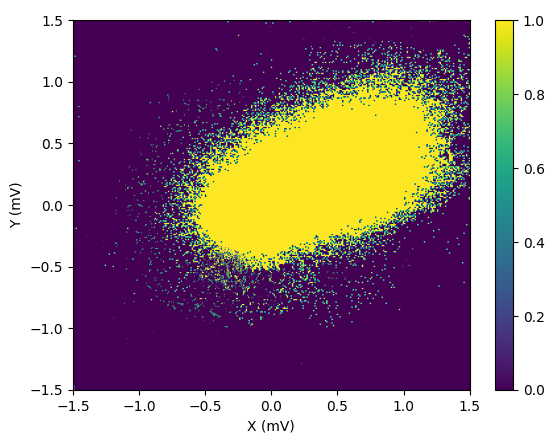
\includegraphics[width=0.65\textwidth]{images/sum_each_beat_all_ecg.png}
    \captionsetup{justification=centering}
    \caption{Representation of the matrix containing the sum of the two-dimensional distributions for each heartbeat across all ECGs following the dataset simplification.}
    \label{fig:sum_each_beat_all_ecg}
\end{figure}

Therefore, a significant improvement can be observed compared to Figure \ref{fig:each_beat_all_ecg} reported in the "Entropy" section (Chapter \ref{chap:materials}, Section \ref{sec:entropia}), achieved through the simplification of the dataset following the application of the clustering algorithm. This further confirms its effectiveness and validity.

\section{Results produced by pre-clustering networks}
\label{sec:network_risultati}

The results presented below unfortunately show that it was not possible to achieve what was initially hoped for, despite implementing and testing numerous neural networks. These results are reported in terms of figures and their corresponding explanations for all three CNNs discussed in the "Convolutional Neural Network" section (Chapter \ref{chap:materials}, Section \ref{sec:network}).

\subsection{First CNN}
\label{subsec:first_cnn_results}

The following Figure \ref{fig:first_cnn_first_plot} illustrates the differences between the two curves of \textit{train} and \textit{val losses}, which respectively represent the measurement of CNN error during training on the training data itself, and the evaluation of CNN error on validation data—separate data on which the CNN has not previously operated. Typically, the \textit{train loss} curve decreases steadily during training as the CNN learns from the training data. However, the \textit{val loss} curve may behave differently: if the \textit{val loss} starts to increase while the \textit{train loss} continues to decrease, it indicates overfitting, meaning the CNN is starting to learn noise in the training data instead of generalizing correctly. In general, the \textit{train} and \textit{val losses} curves can guide the choice of the best CNN. The goal is to find a balance between minimizing error on training data (\textit{low train loss}) and maintaining good generalization on validation data (\textit{low val loss}):

\begin{figure}[H]
    \centering
    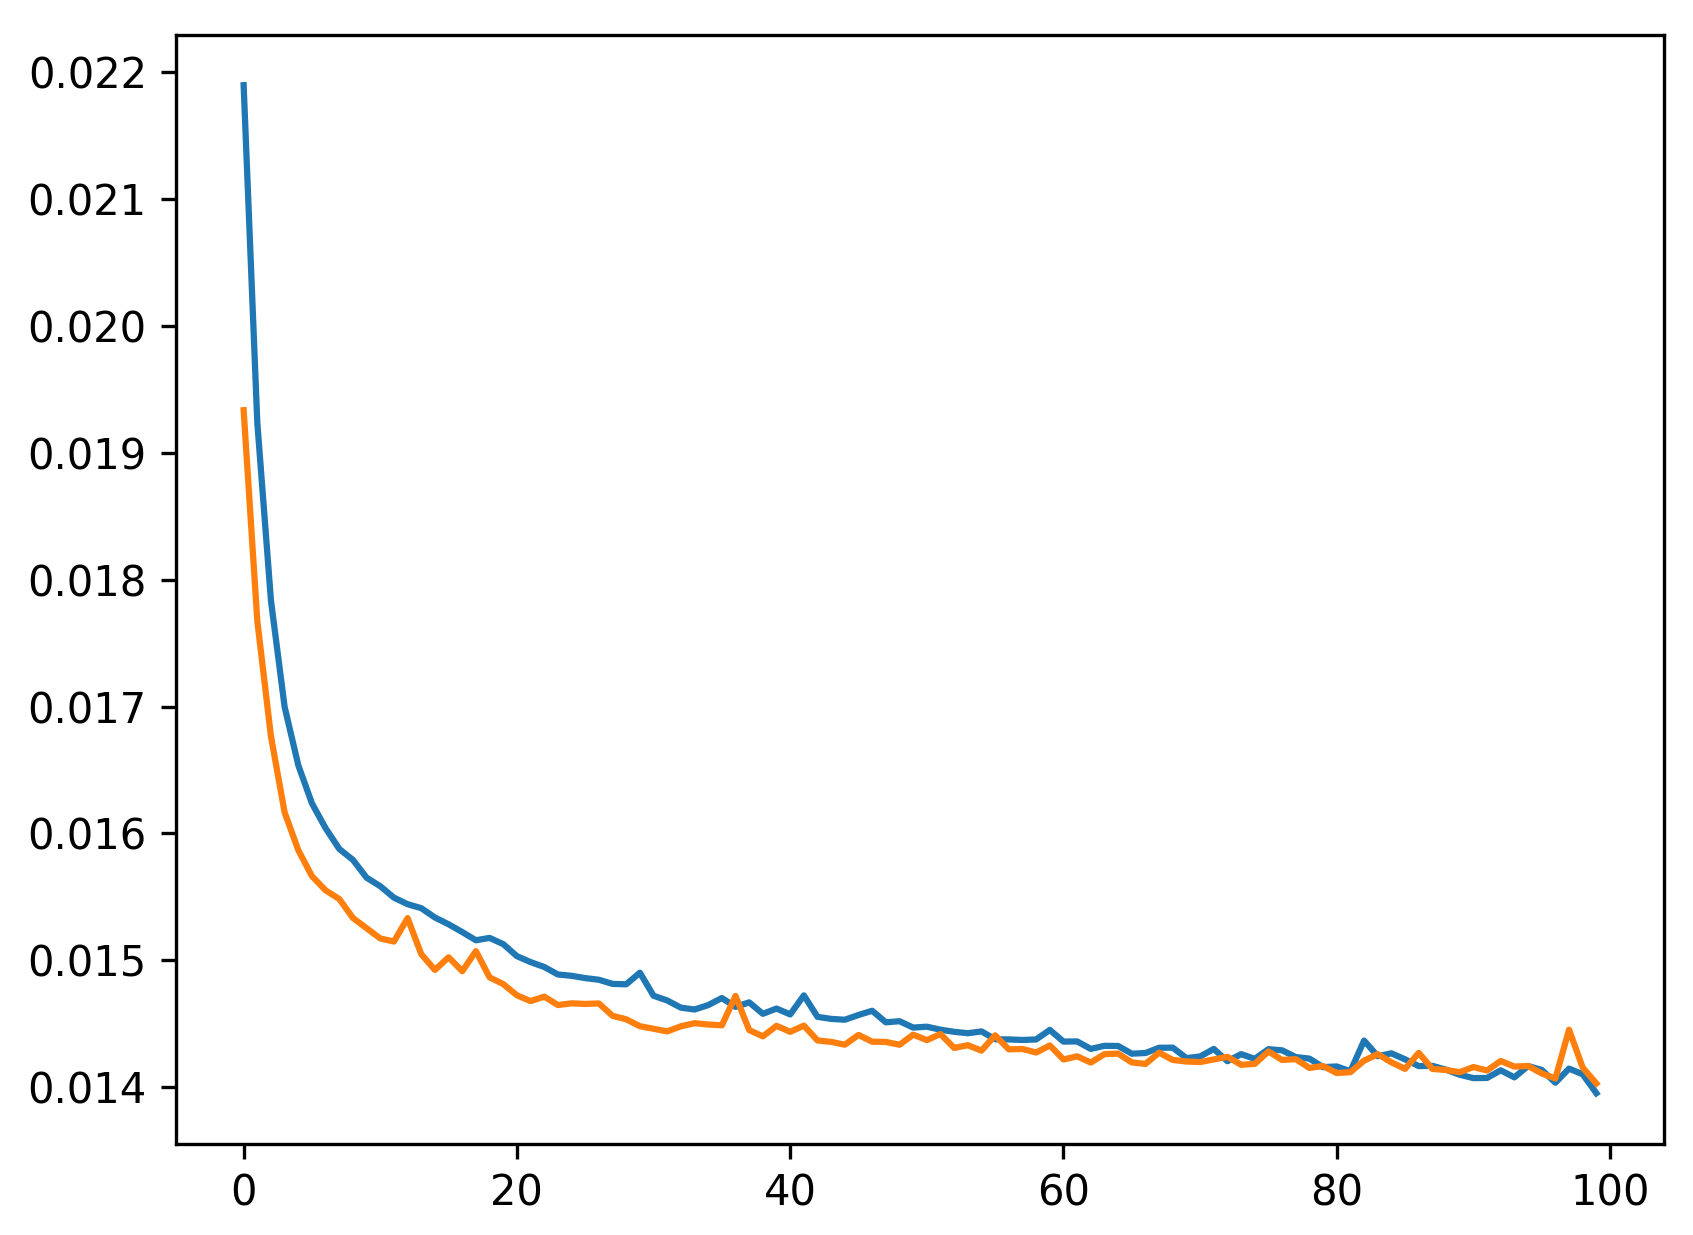
\includegraphics[width=0.65\textwidth]{images/first_cnn_first_plot.png}
    \captionsetup{justification=centering}
    \caption{Differences between the \textit{val loss} curve (in blue) and \textit{train loss} curve (in orange) for the first implemented and tested CNN.}
    \label{fig:first_cnn_first_plot}
\end{figure}

Despite both \textit{train loss} and \textit{val loss} curves showing positive trends with decreasing values, the plots obtained after completing the tests did not yield the initially expected results, as can be inferred from the following Figure \ref{fig:first_cnn_second_plot}. Unfortunately, the figure illustrates that the two graphs hardly overlap:

\begin{figure}[H]
    \centering
    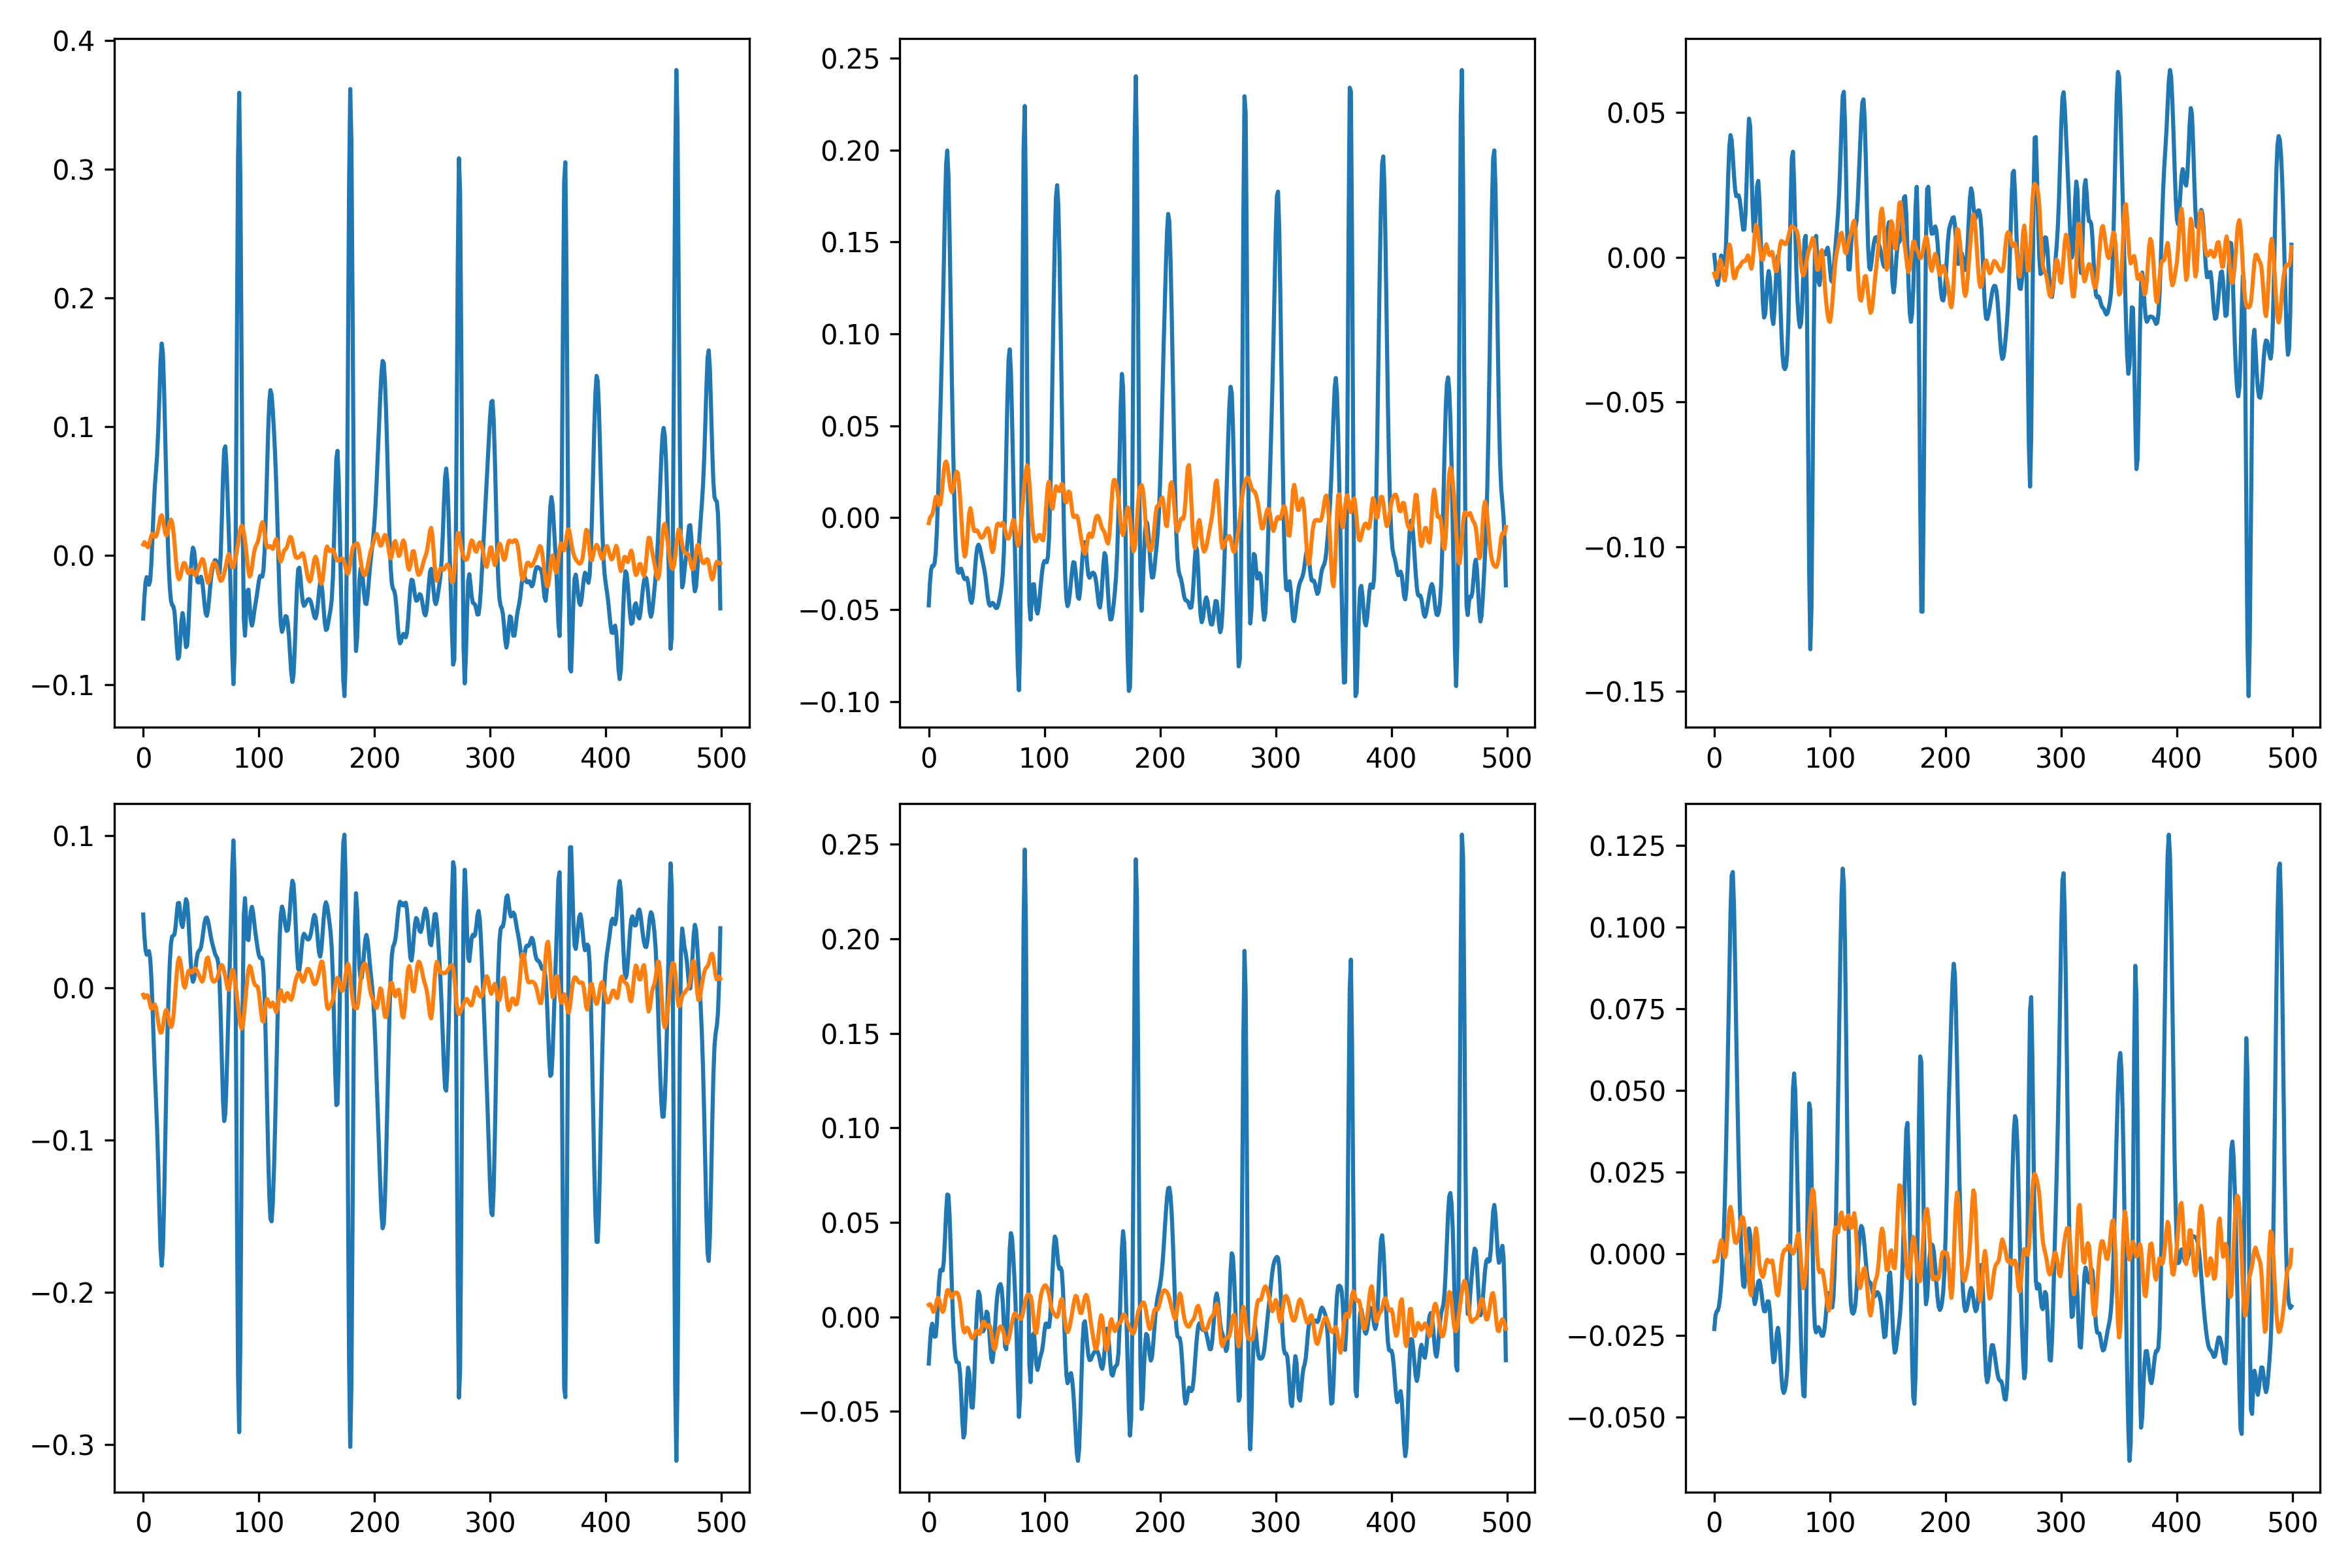
\includegraphics[width=0.85\textwidth]{images/first_cnn_second_plot.png}
    \captionsetup{justification=centering}
    \caption{Results obtained from the tests conducted with the first implemented and tested CNN.}
    \label{fig:first_cnn_second_plot}
\end{figure}


\subsection{Second CNN}
\label{subsec:second_cnn_results}

Similarly, the following Figure \ref{fig:second_cnn_first_plot} illustrates the differences between the \textit{train} and \textit{val losses} curves for the CNN mentioned immediately above. It can be observed that despite a significant increase in the complexity of the CNN, the \textit{val loss} curve does not decrease consistently throughout the training period. Instead, it decreases only initially for a short period before slightly increasing and stabilizing towards the end around a certain value. This demonstrates that increasing the complexity of the CNN does not necessarily lead to improved test results and, in fact, often results in significant deterioration, as seen in this case:

\begin{figure}[H]
    \centering
    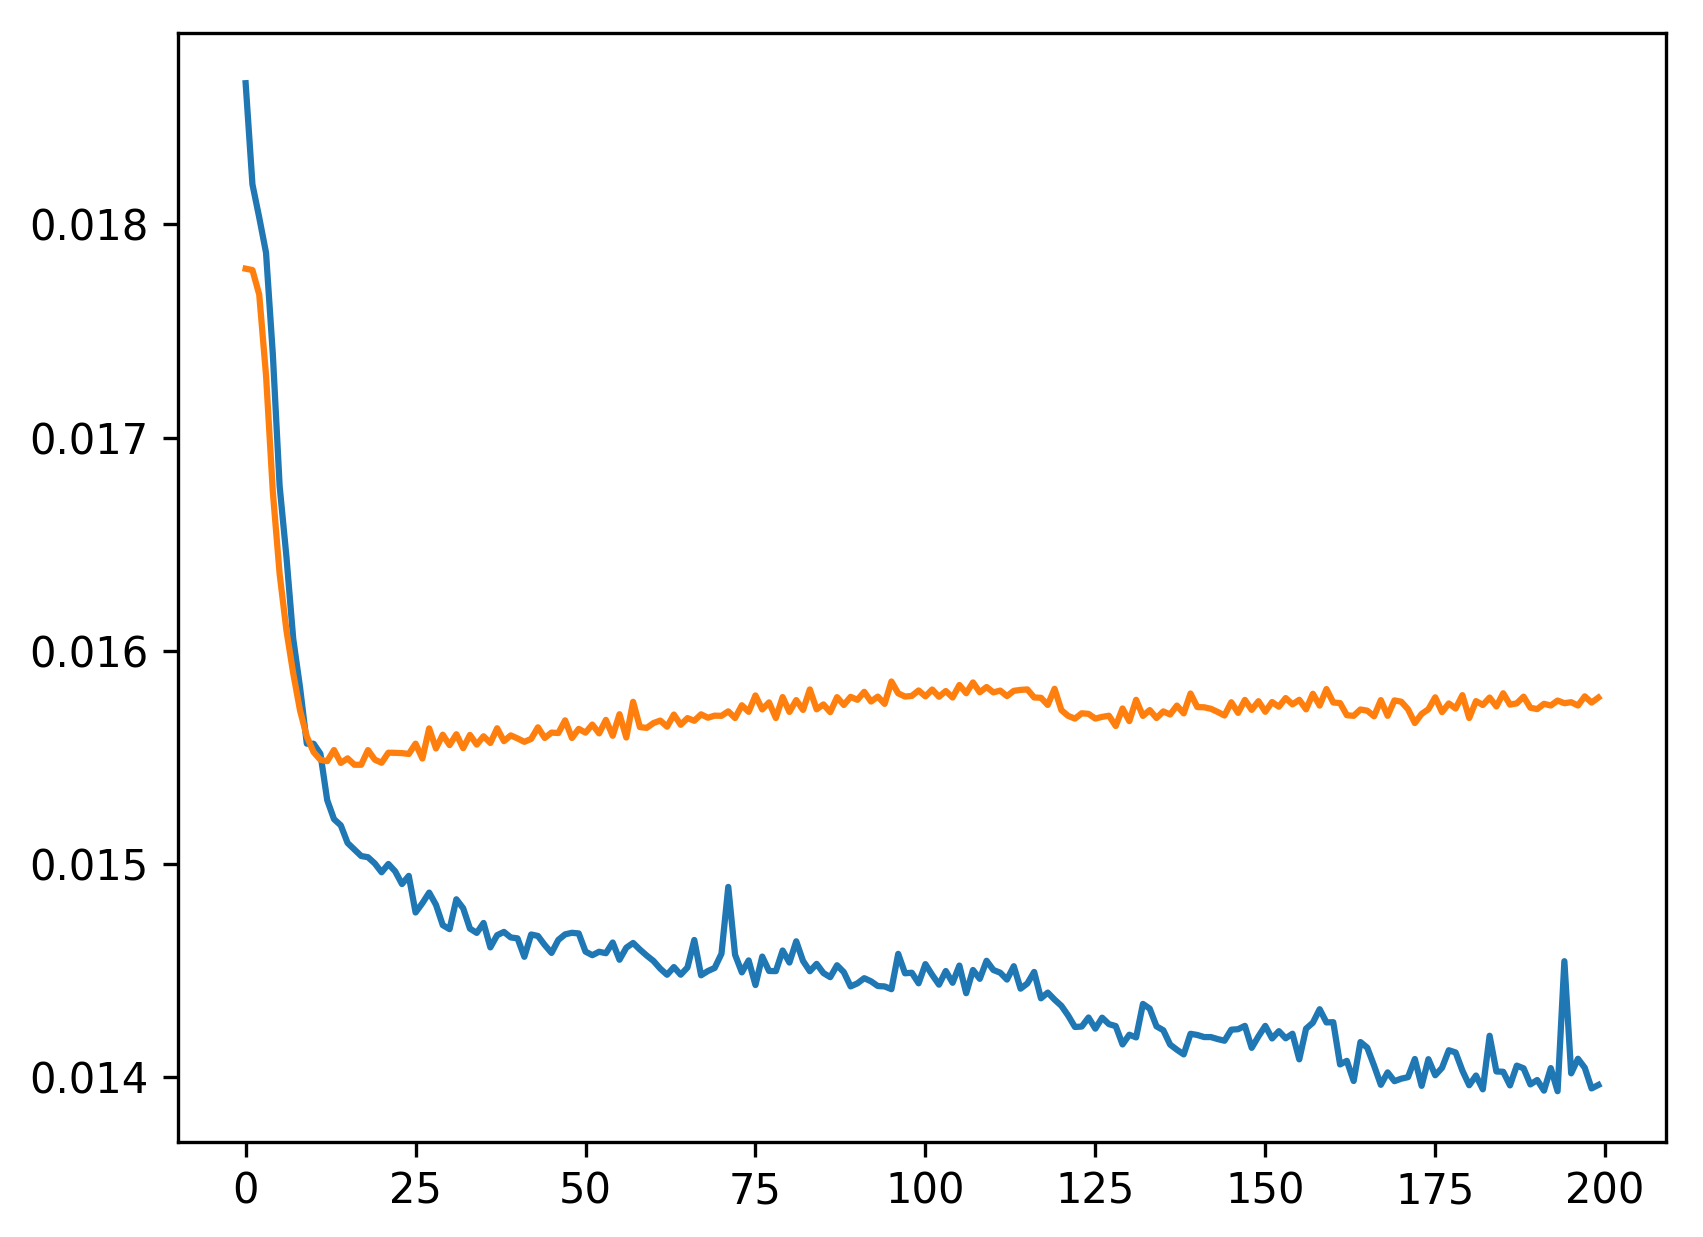
\includegraphics[width=0.65\textwidth]{images/second_cnn_first_plot.png}
    \captionsetup{justification=centering}
    \caption{Differences between the \textit{val loss} curve (in blue) and \textit{train loss} curve (in orange) for the second implemented and tested CNN.}
    \label{fig:second_cnn_first_plot}
\end{figure}

In this case, despite the \textit{train} and \textit{val losses} curves resulting in much worse performance compared to the curves of the first CNN mentioned earlier, it can be observed from the following Figures \ref{fig:second_cnn_second_plot_0} and \ref{fig:second_cnn_second_plot_1} that the plots obtained after completing the tests yielded results much closer to what one would expect compared to the plots obtained from testing the first CNN. However, once again, the results were not satisfactory in terms of performance, leading to further modifications to the CNN in search of better results:

\begin{figure}[H]
    \centering
    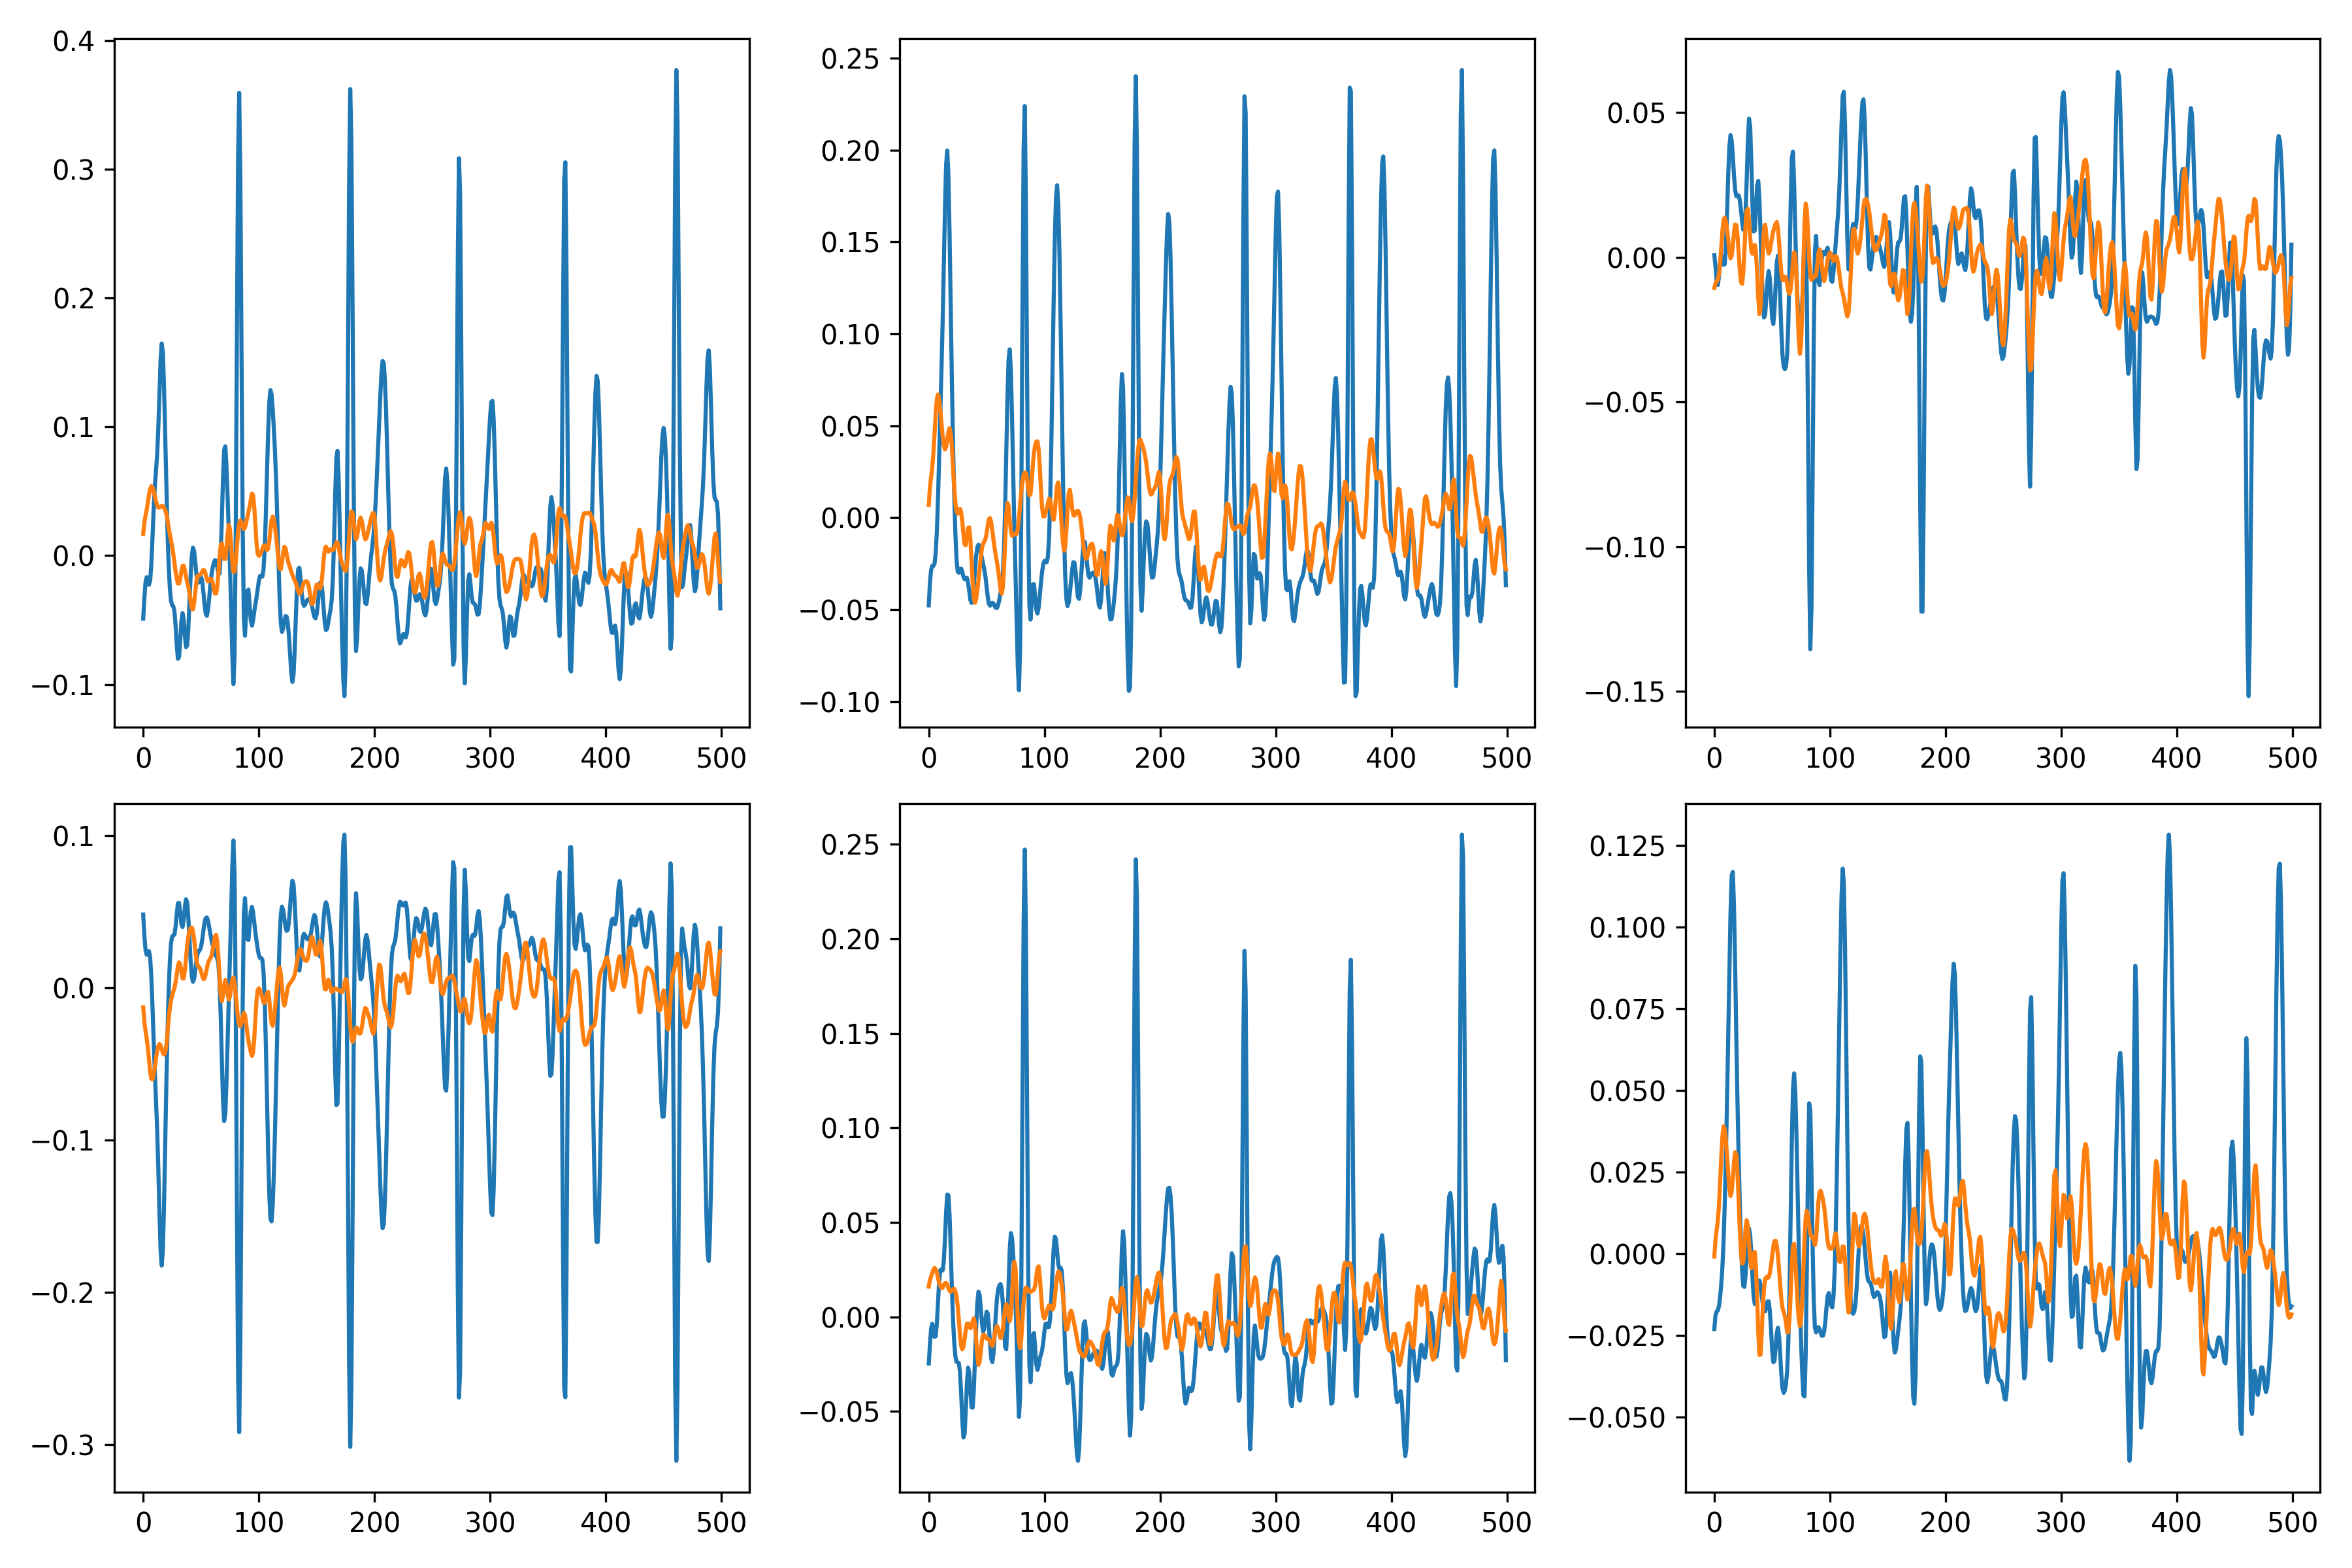
\includegraphics[width=0.85\textwidth]{images/second_cnn_second_plot_0.png}
    \captionsetup{justification=centering}
    \caption{Results obtained from the tests conducted with the second implemented and tested CNN.}
    \label{fig:second_cnn_second_plot_0}
\end{figure}
\begin{figure}[H]
    \centering
    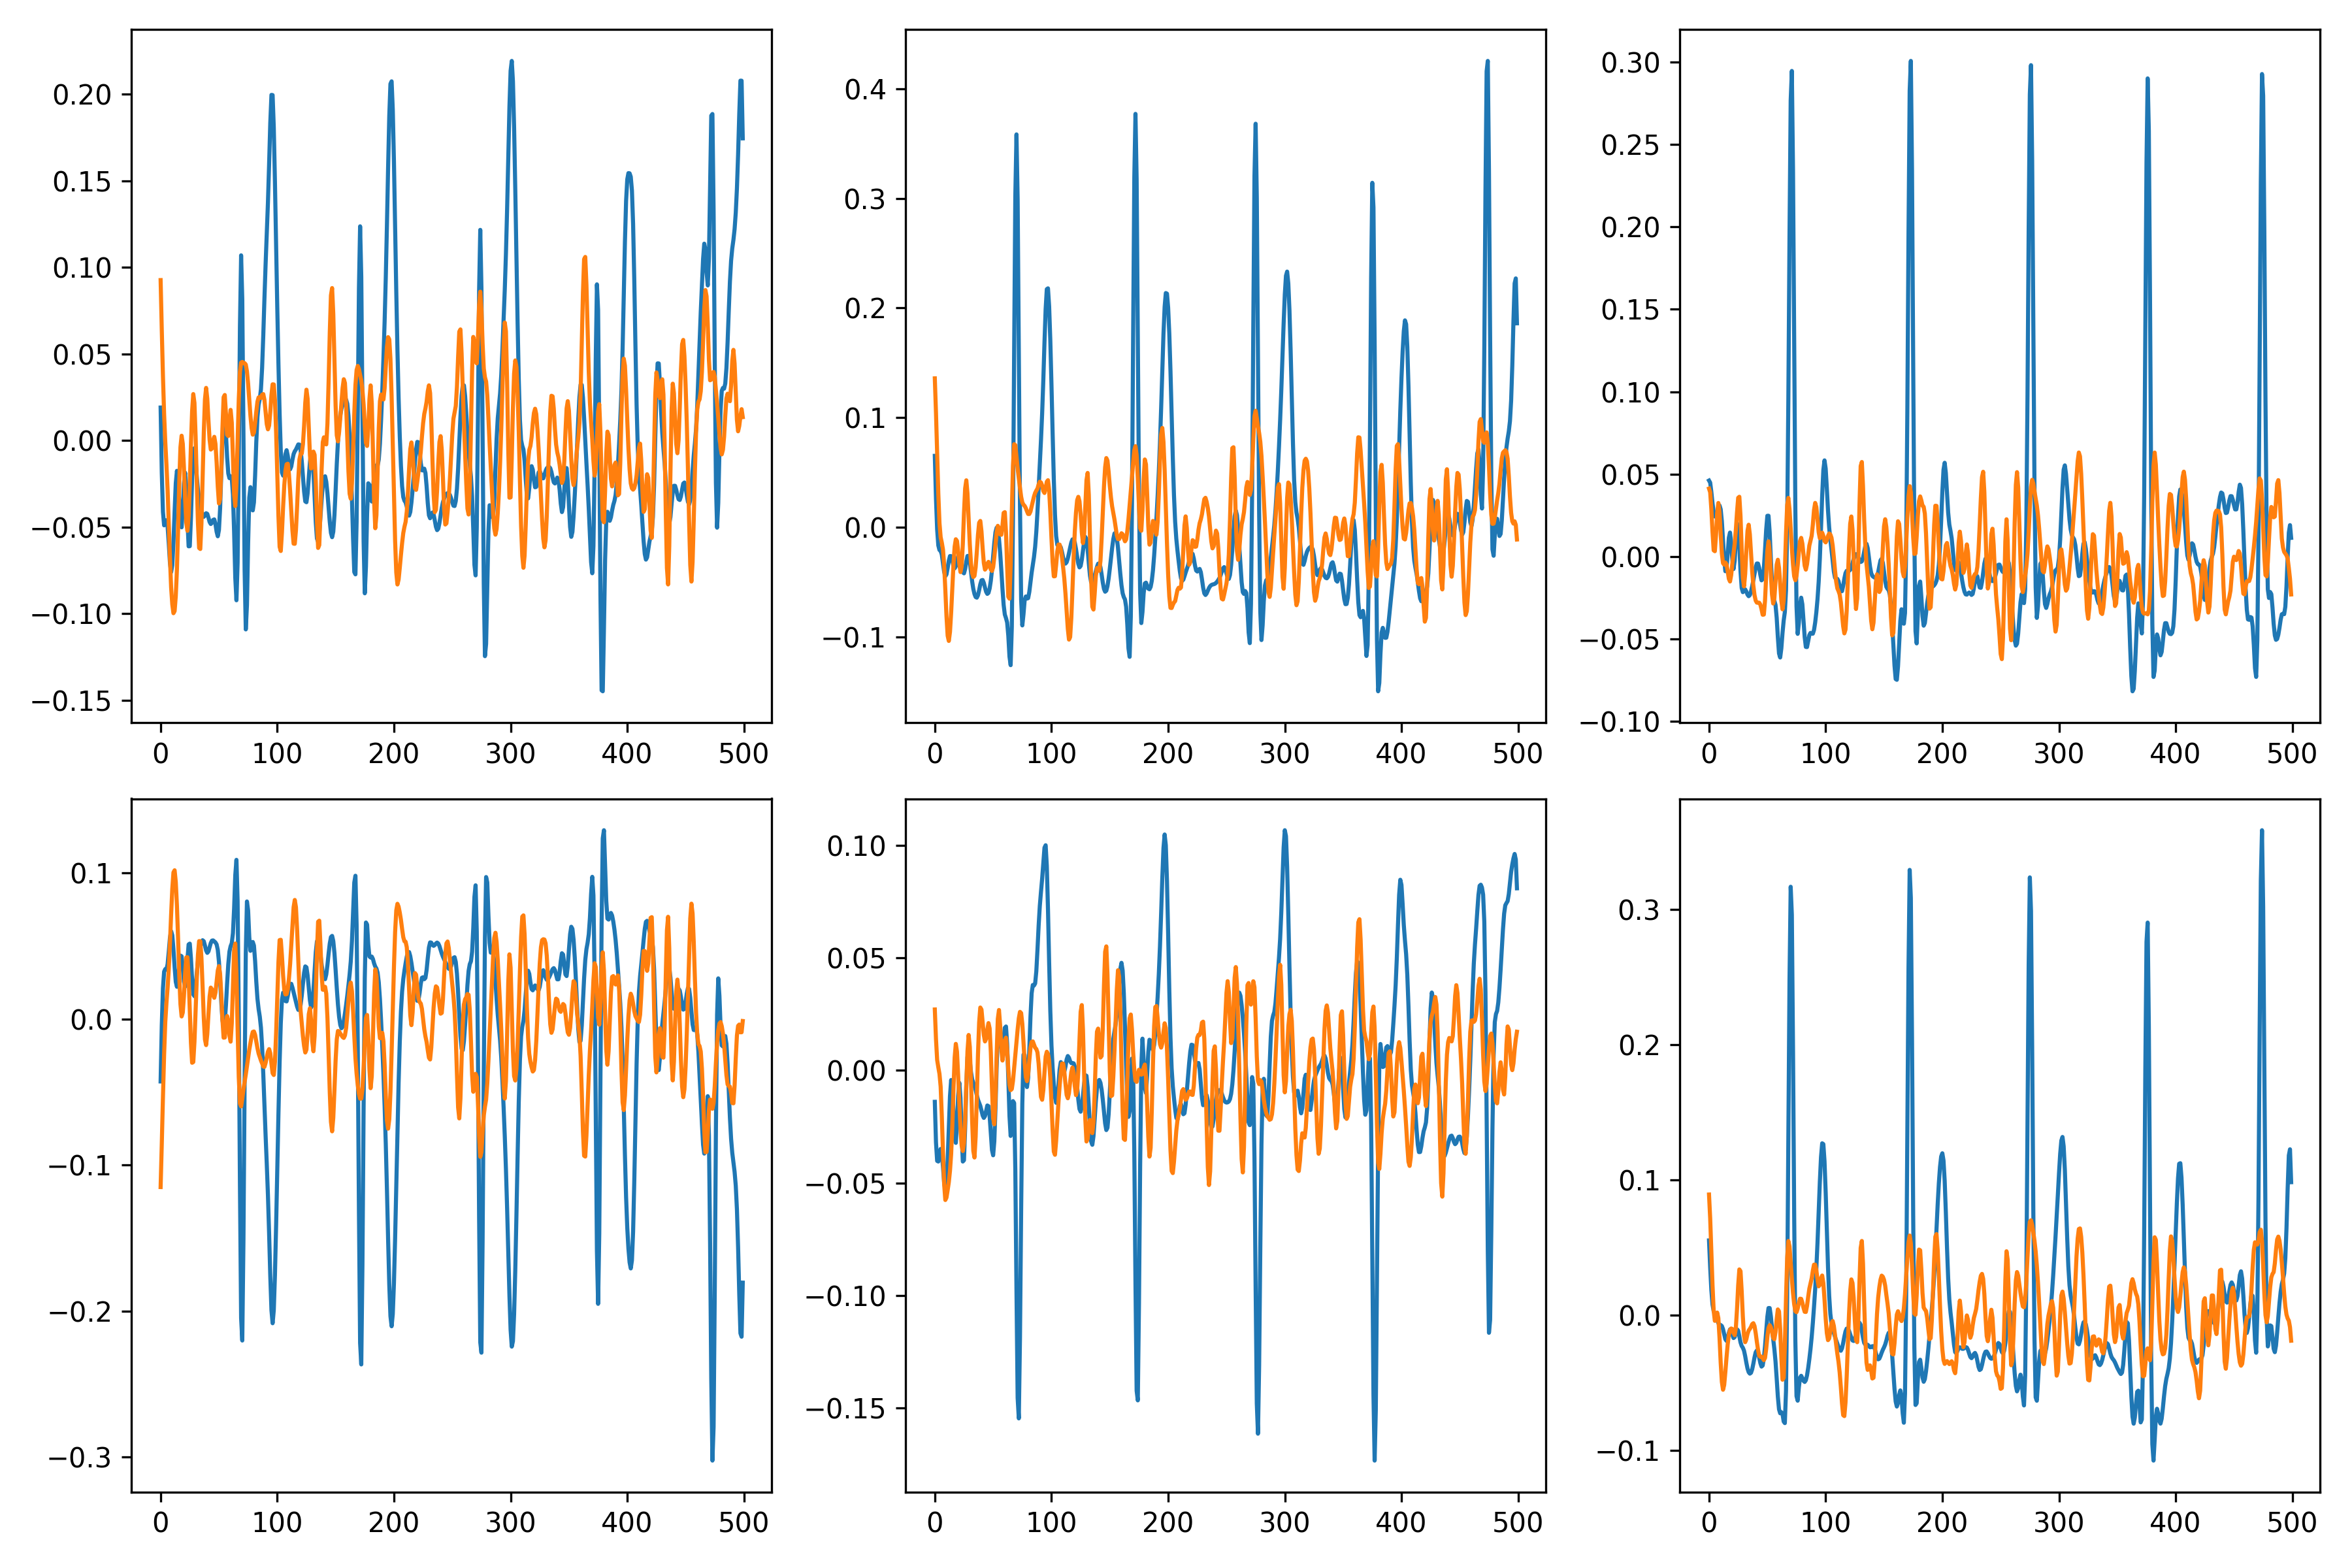
\includegraphics[width=0.85\textwidth]{images/second_cnn_second_plot_1.png}
    \captionsetup{justification=centering}
    \caption{Results obtained from the tests conducted with the second implemented and tested CNN.}
    \label{fig:second_cnn_second_plot_1}
\end{figure}


\subsection{Third CNN}
\label{subsec:third_cnn_results}

Finally, below is the last Figure \ref{fig:third_cnn_first_plot}, illustrating the differences between the \textit{train} and \textit{val losses} curves for the CNN mentioned just above. In this case, both curves initially decrease over a period of time, stabilizing almost entirely at the same value until the end of the tests. However, there is a sharp increase followed immediately by an equally sharp decrease towards the end of the test period on the x-axis of the \textit{train loss} curve:

\begin{figure}[H]
    \centering
    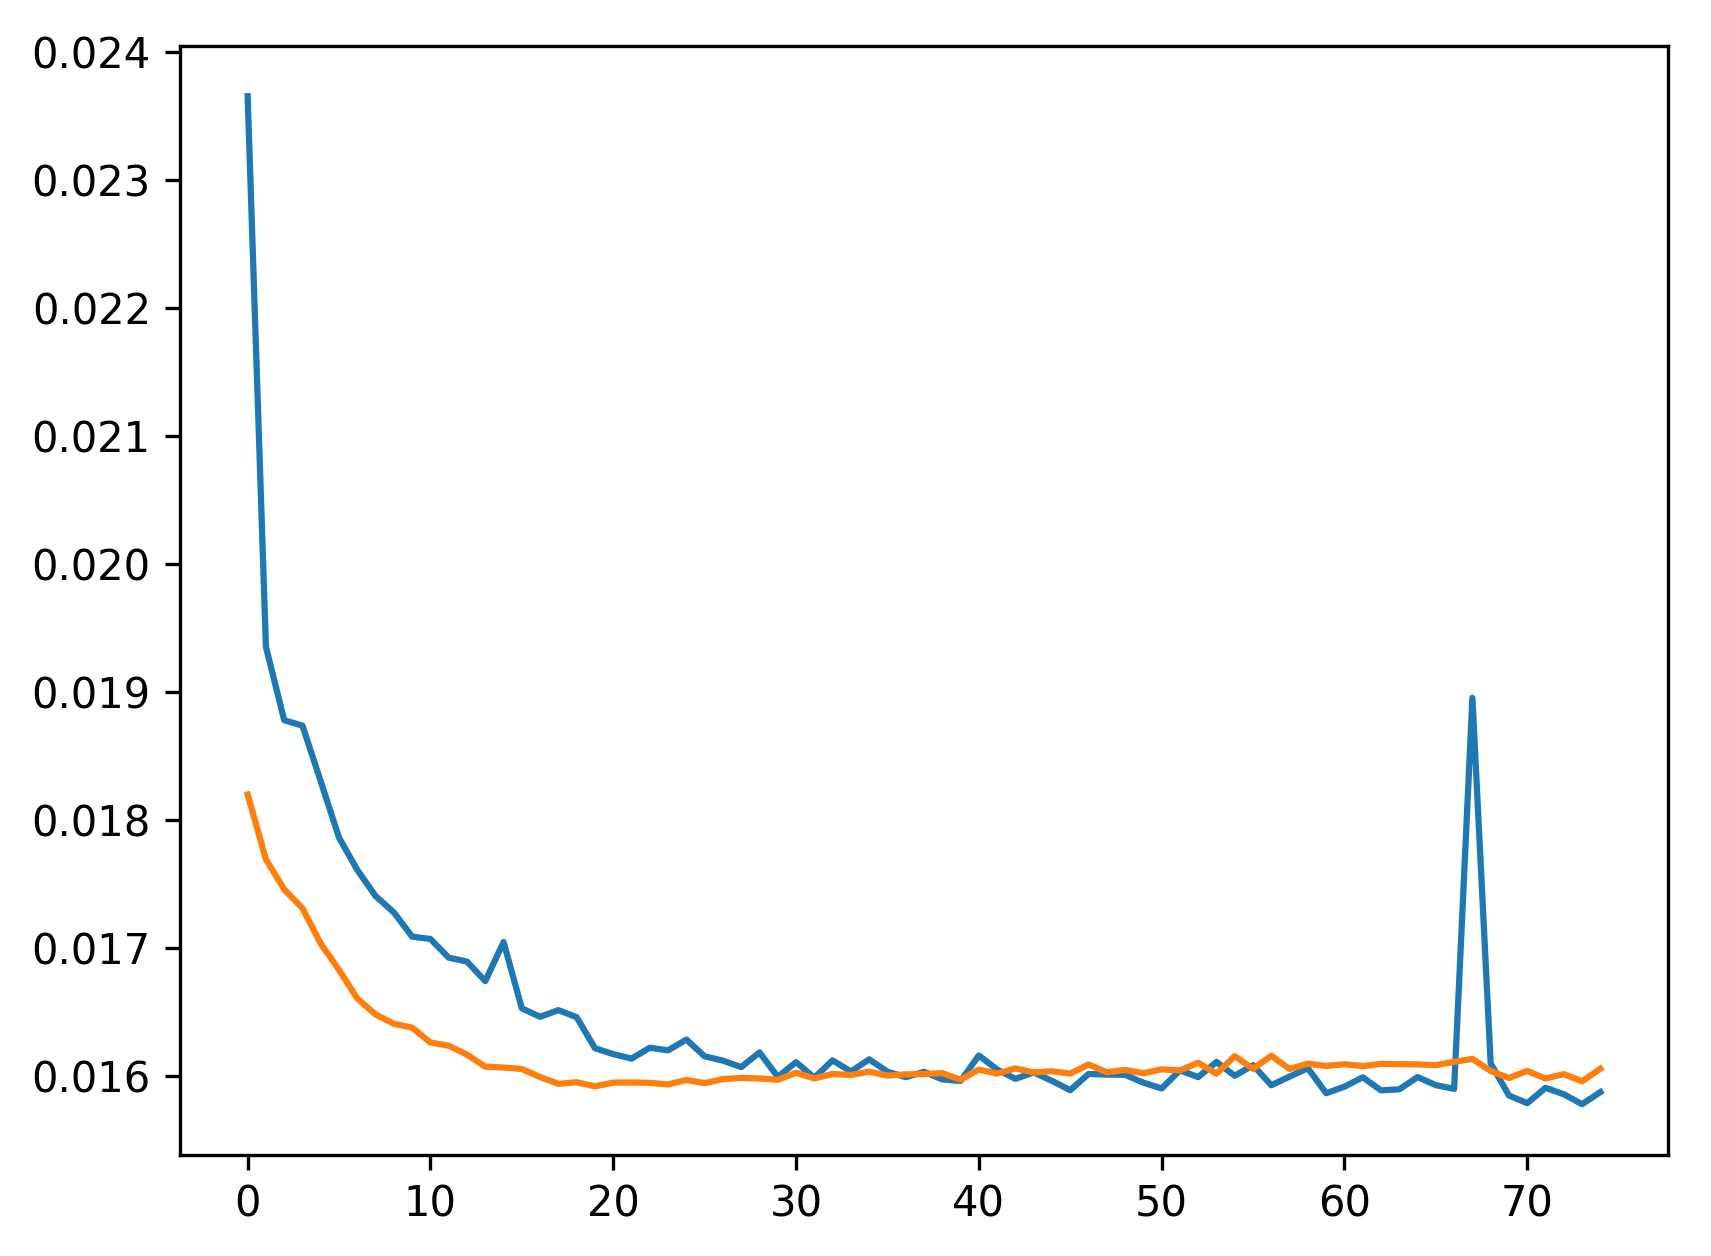
\includegraphics[width=0.65\textwidth]{images/third_cnn_first_plot.png}
    \captionsetup{justification=centering}
    \caption{Differences between the \textit{val loss} curve (in blue) and \textit{train loss} curve (in orange) for the third implemented and tested CNN.}
    \label{fig:third_cnn_first_plot}
\end{figure}

Upon reviewing the \textit{train} and \textit{val losses} curves, it can be observed from the following Figures \ref{fig:third_cnn_second_plot_0} and \ref{fig:third_cnn_second_plot_1} how the plots obtained after the tests resulted once again very close to what one would expect, with the lines overlapping at multiple points. However, unfortunately, they are still not completely satisfactory in terms of results:

\begin{figure}[H]
    \centering
    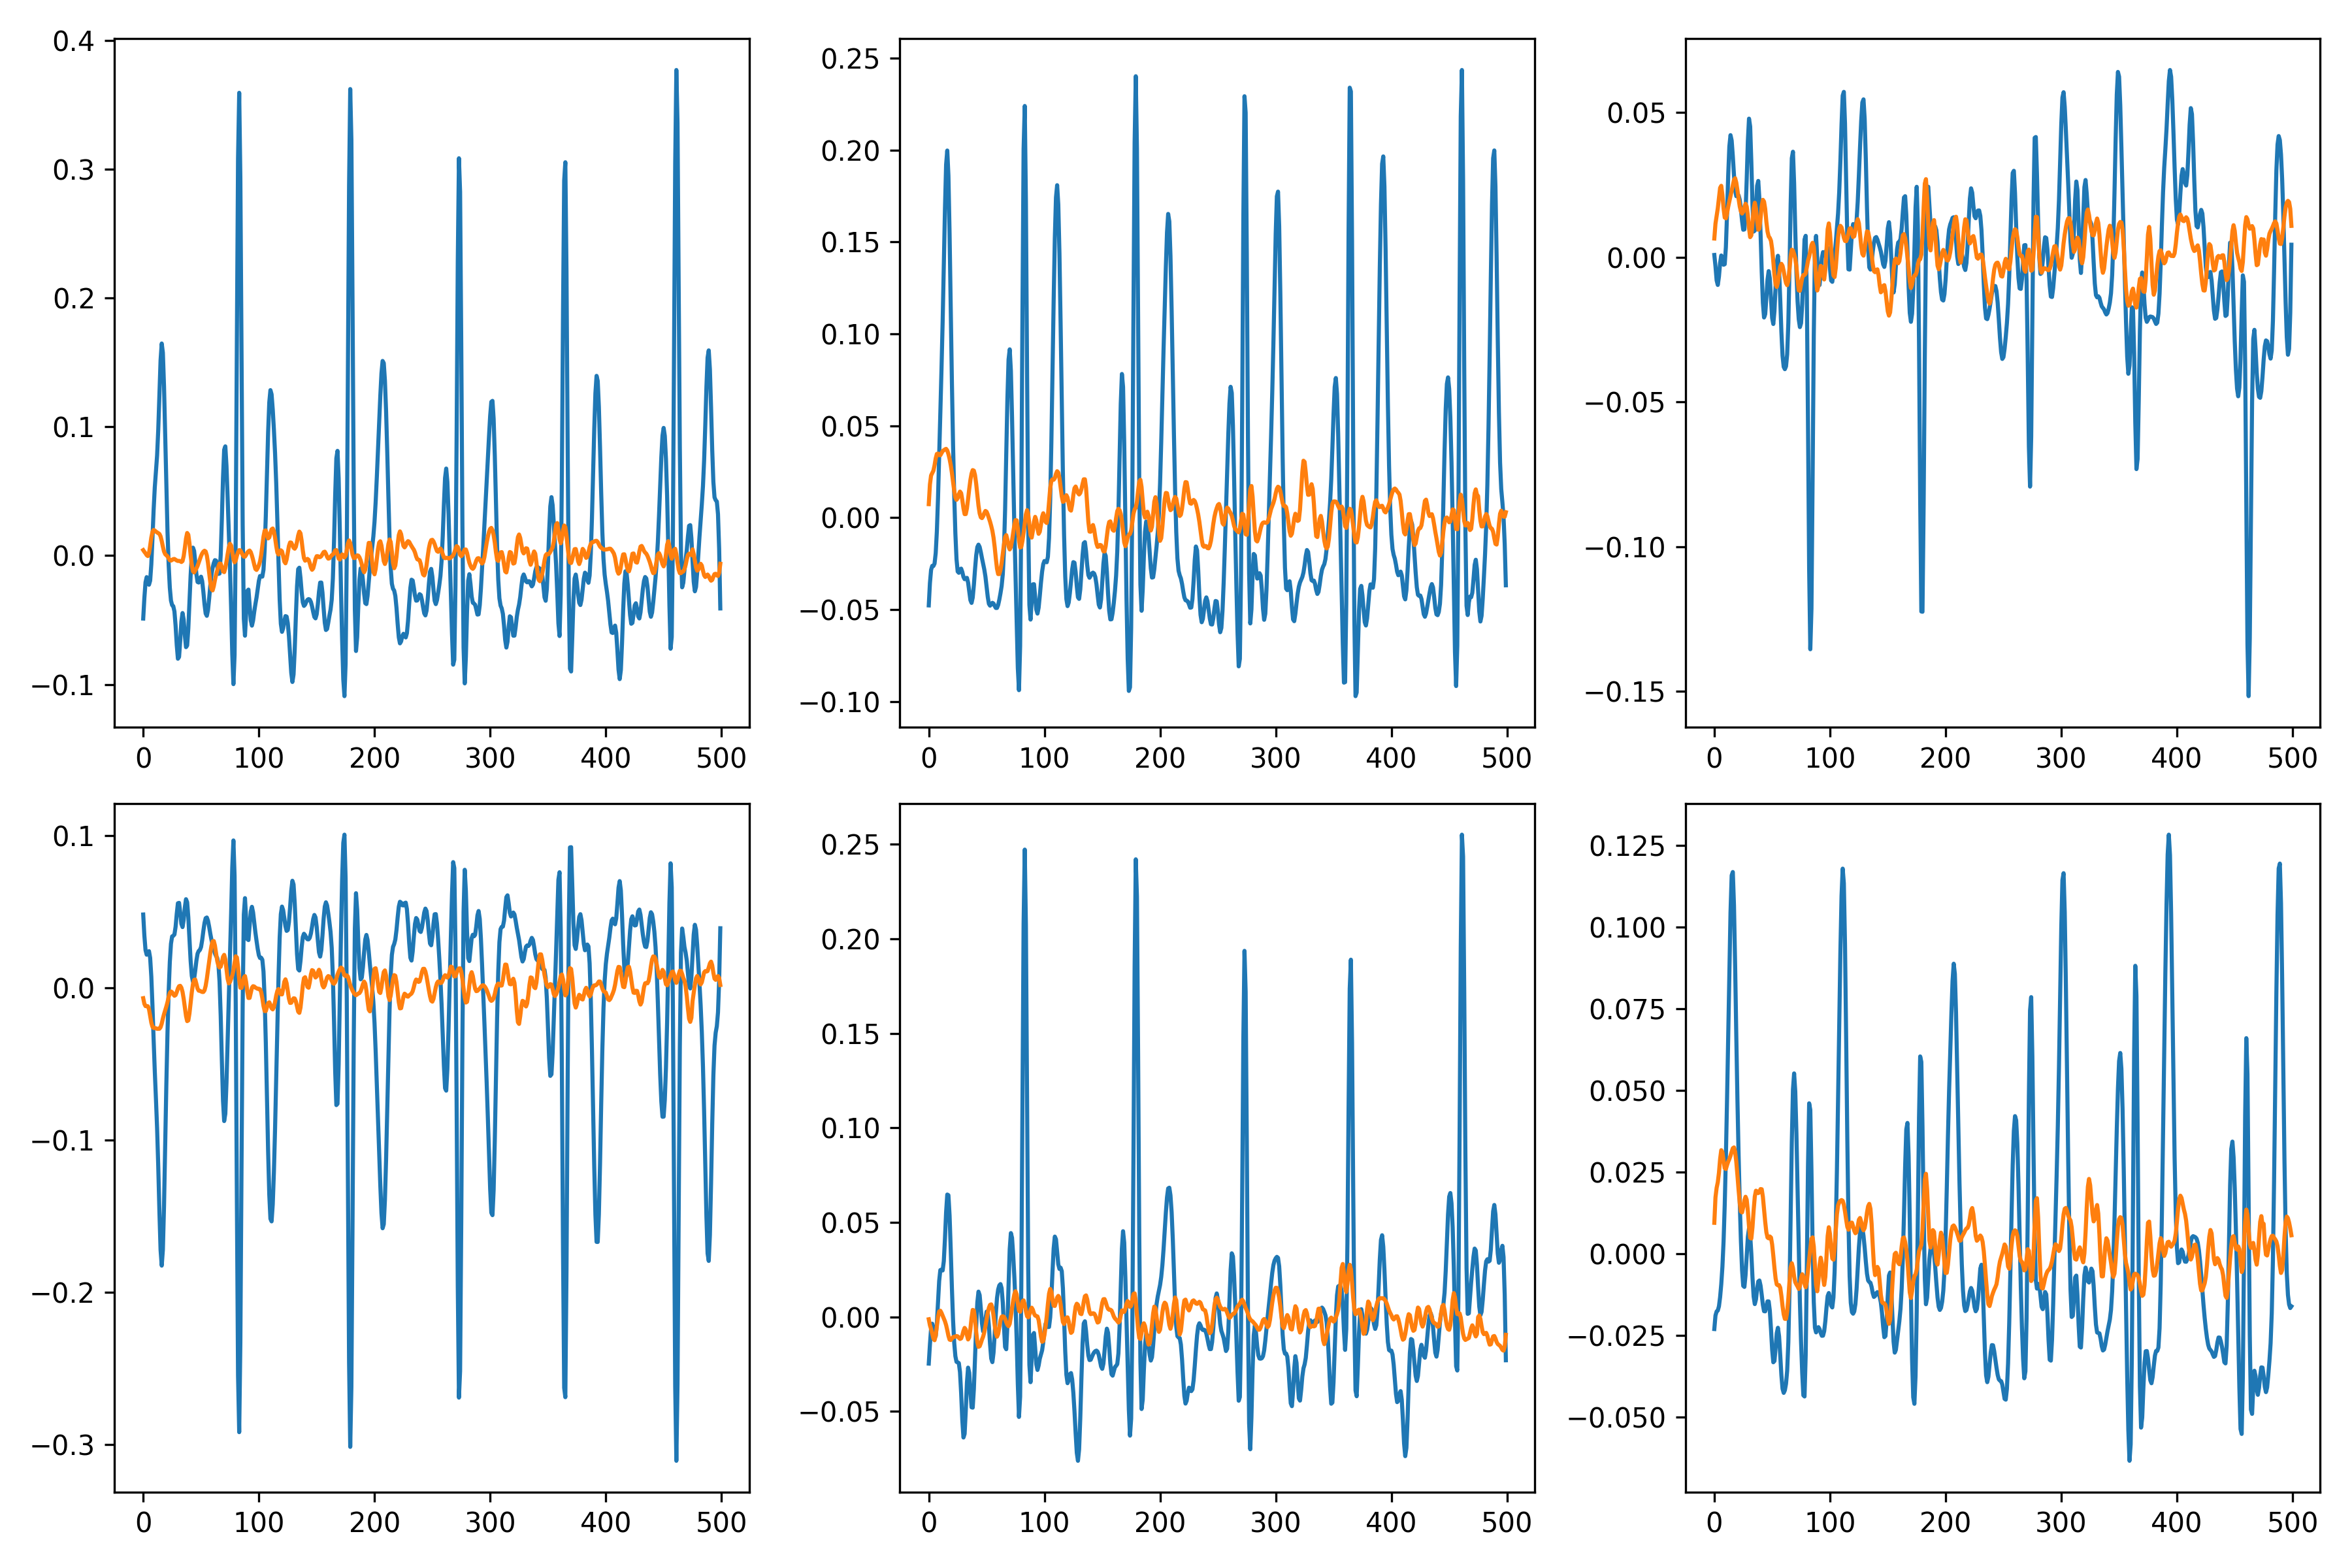
\includegraphics[width=0.85\textwidth]{images/third_cnn_second_plot_0.png}
    \captionsetup{justification=centering}
    \caption{Results obtained from the tests conducted with the third implemented and tested CNN.}
    \label{fig:third_cnn_second_plot_0}
\end{figure}
\begin{figure}[H]
    \centering
    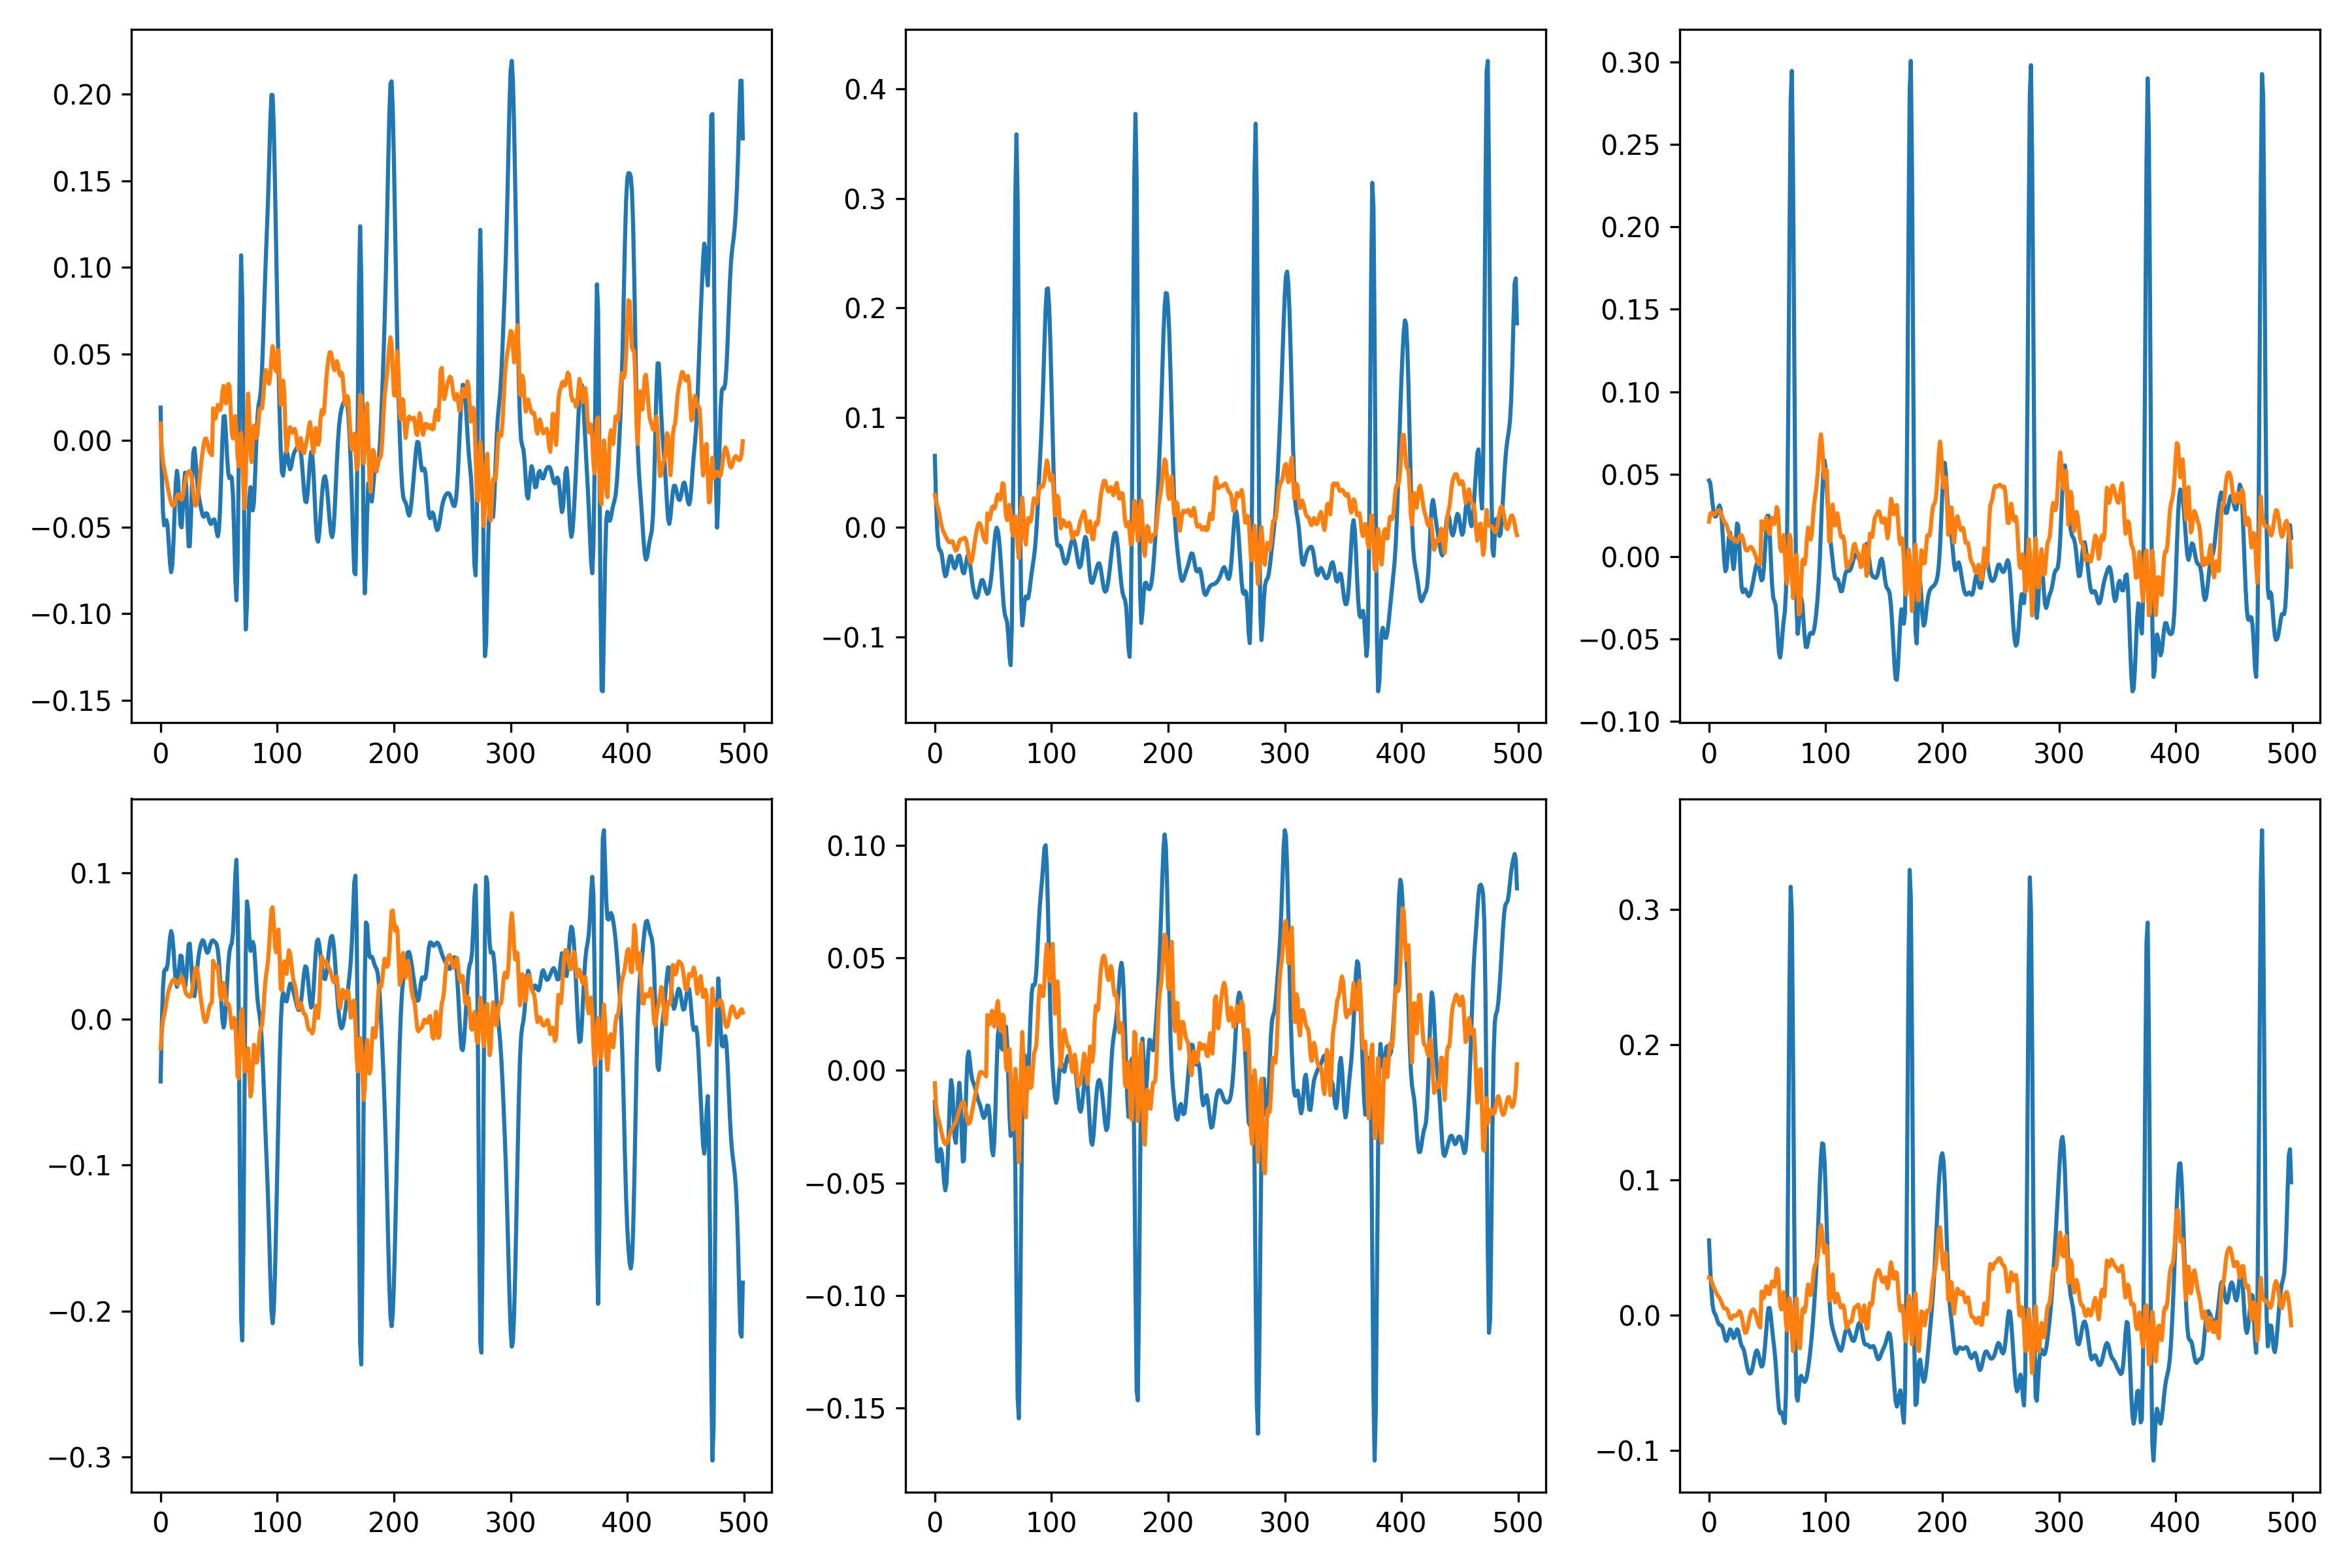
\includegraphics[width=0.85\textwidth]{images/third_cnn_second_plot_1.png}
    \captionsetup{justification=centering}
    \caption{Results obtained from the tests conducted with the third implemented and tested CNN.}
    \label{fig:third_cnn_second_plot_1}
\end{figure}

\section{Results produced by post-clustering networks}
\label{sec:clustering_risultati}

Despite in theory the application of the clustering algorithm should have significantly improved the results produced by the tests of the various networks, as can be seen from figures \ref{fig:first_cnn_result_second_plot_0}, \ref{fig:first_cnn_result_second_plot_1}, \ref{fig:second_cnn_result_second_plot_0}, and \ref{fig:second_cnn_result_second_plot_1} reported below, once again these have not proven to be completely satisfactory, although they are still better compared to the previous results, indicating significant progress due to dataset simplification:

\begin{figure}[H]
    \centering
    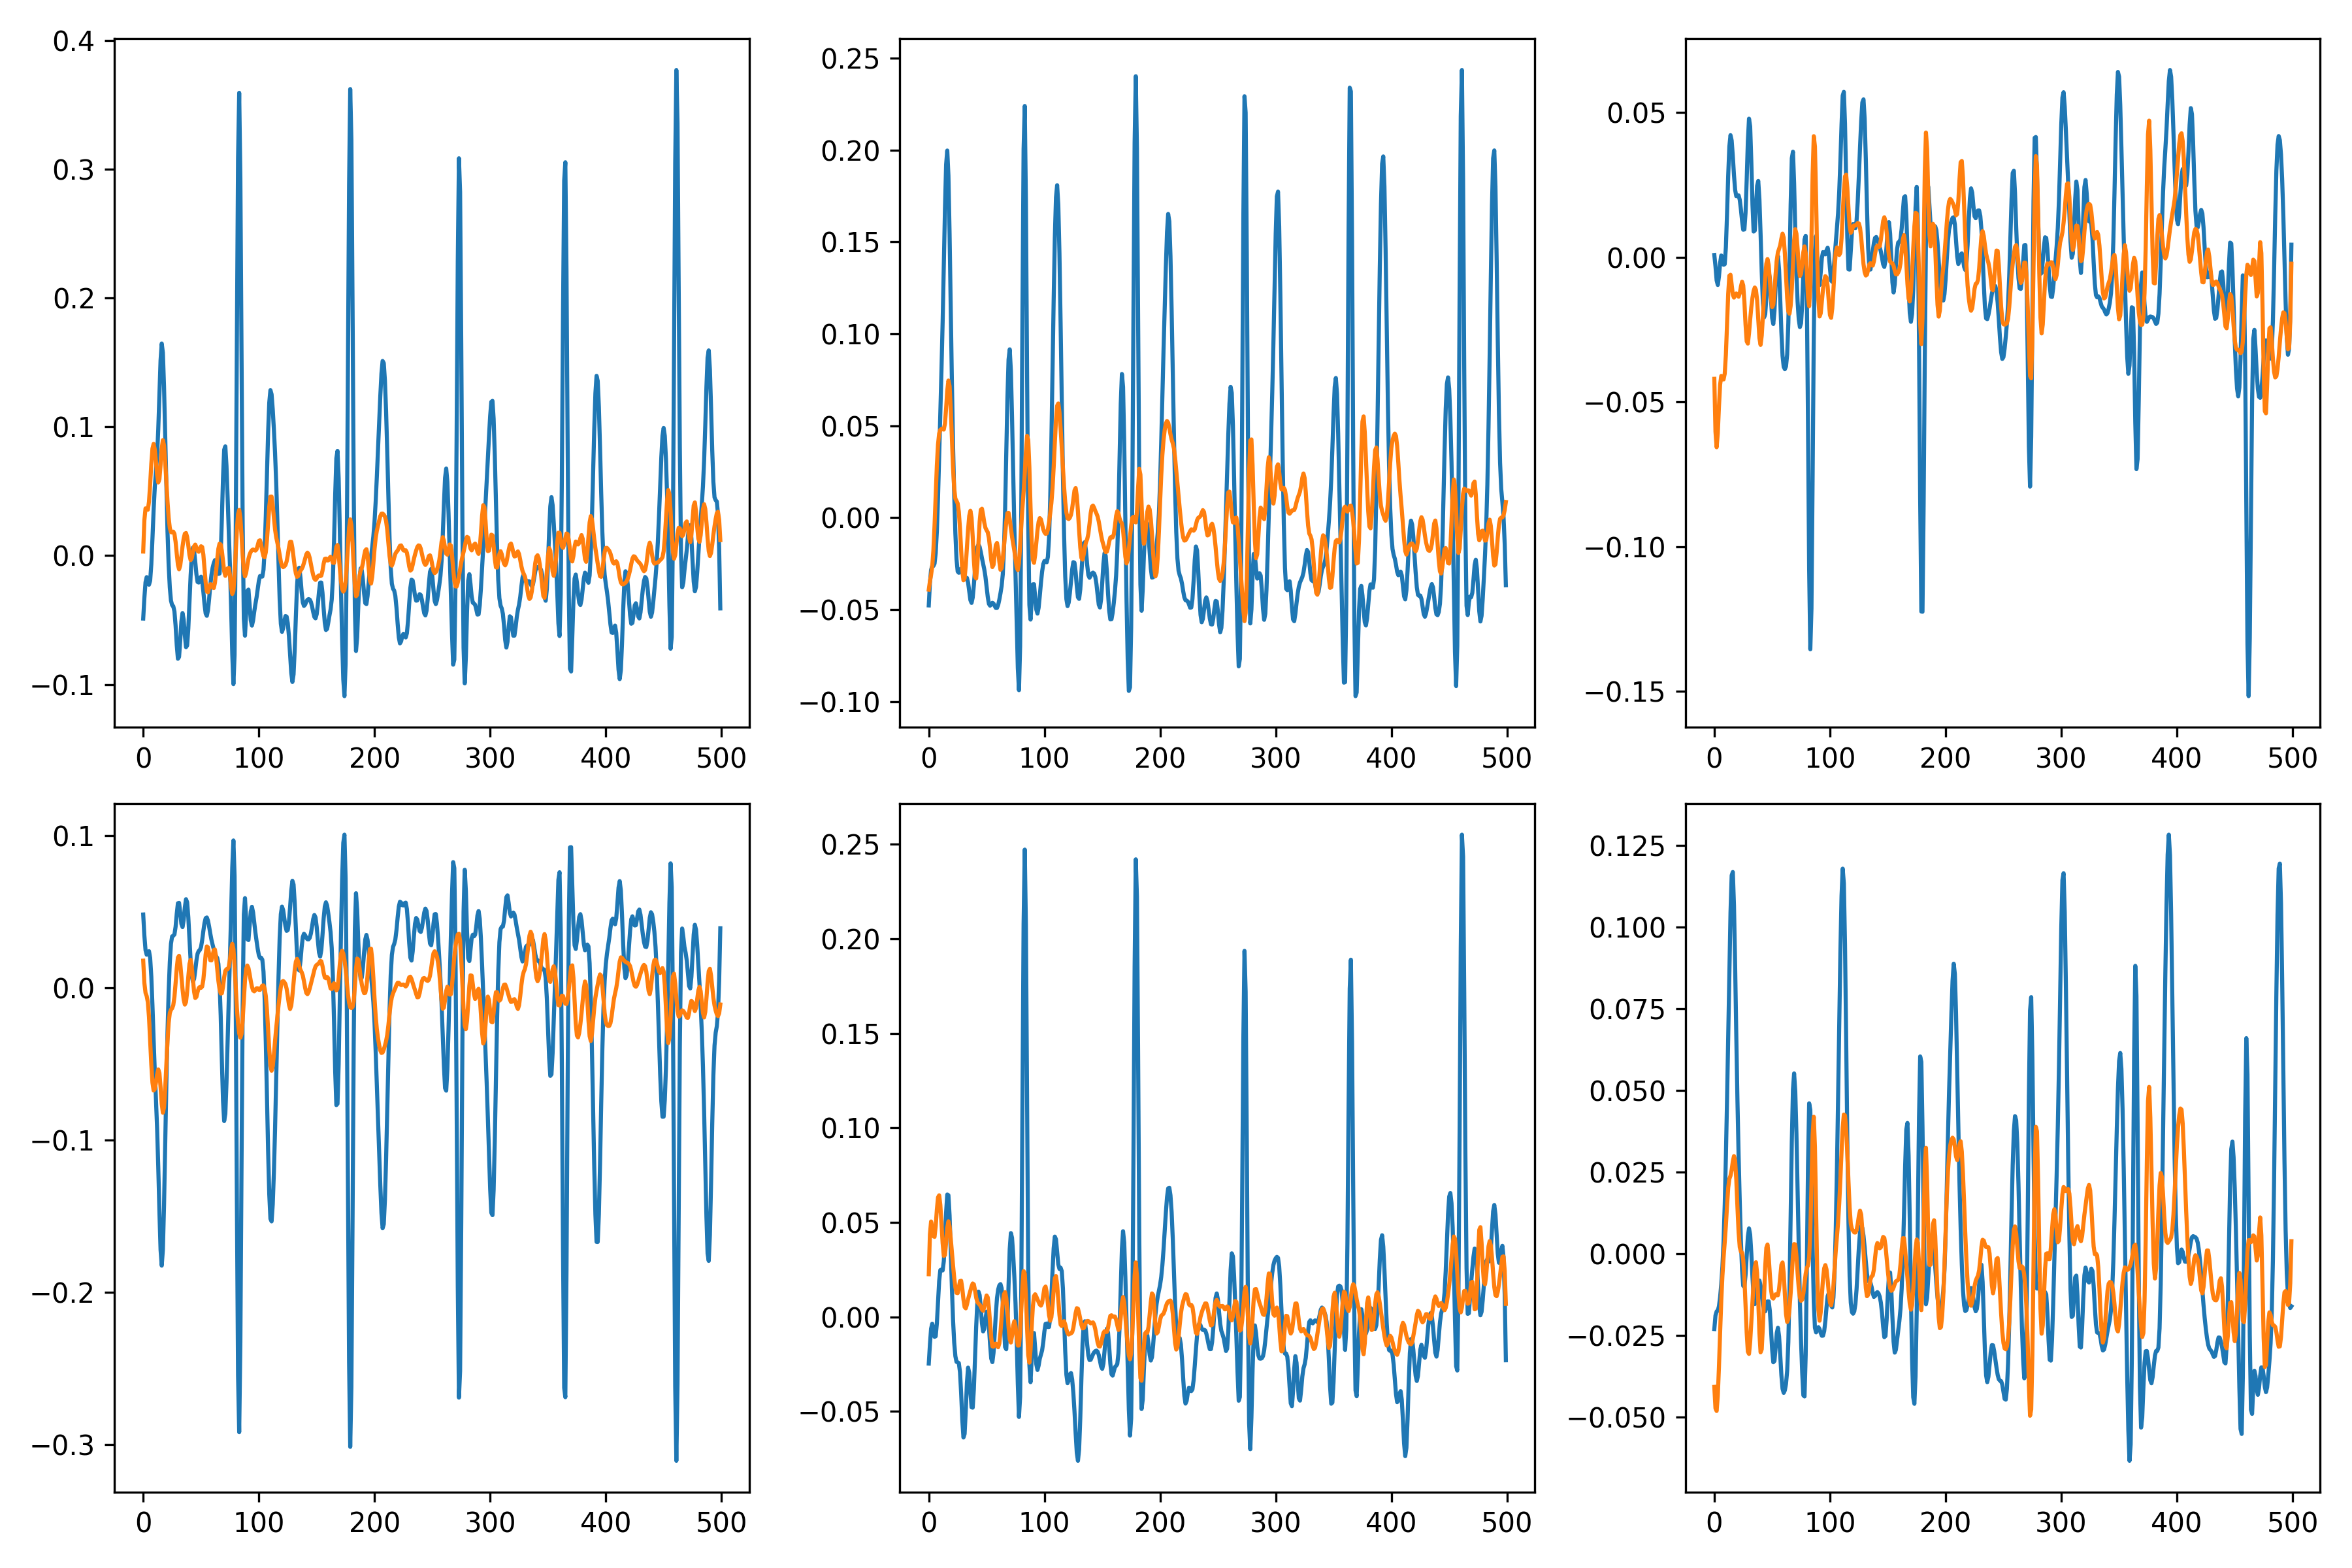
\includegraphics[width=0.85\textwidth]{images/first_cnn_result_second_plot_0.png}
    \captionsetup{justification=centering}
    \caption{Results obtained from the tests conducted following dataset simplification.}
    \label{fig:first_cnn_result_second_plot_0}
\end{figure}
\begin{figure}[H]
    \centering
    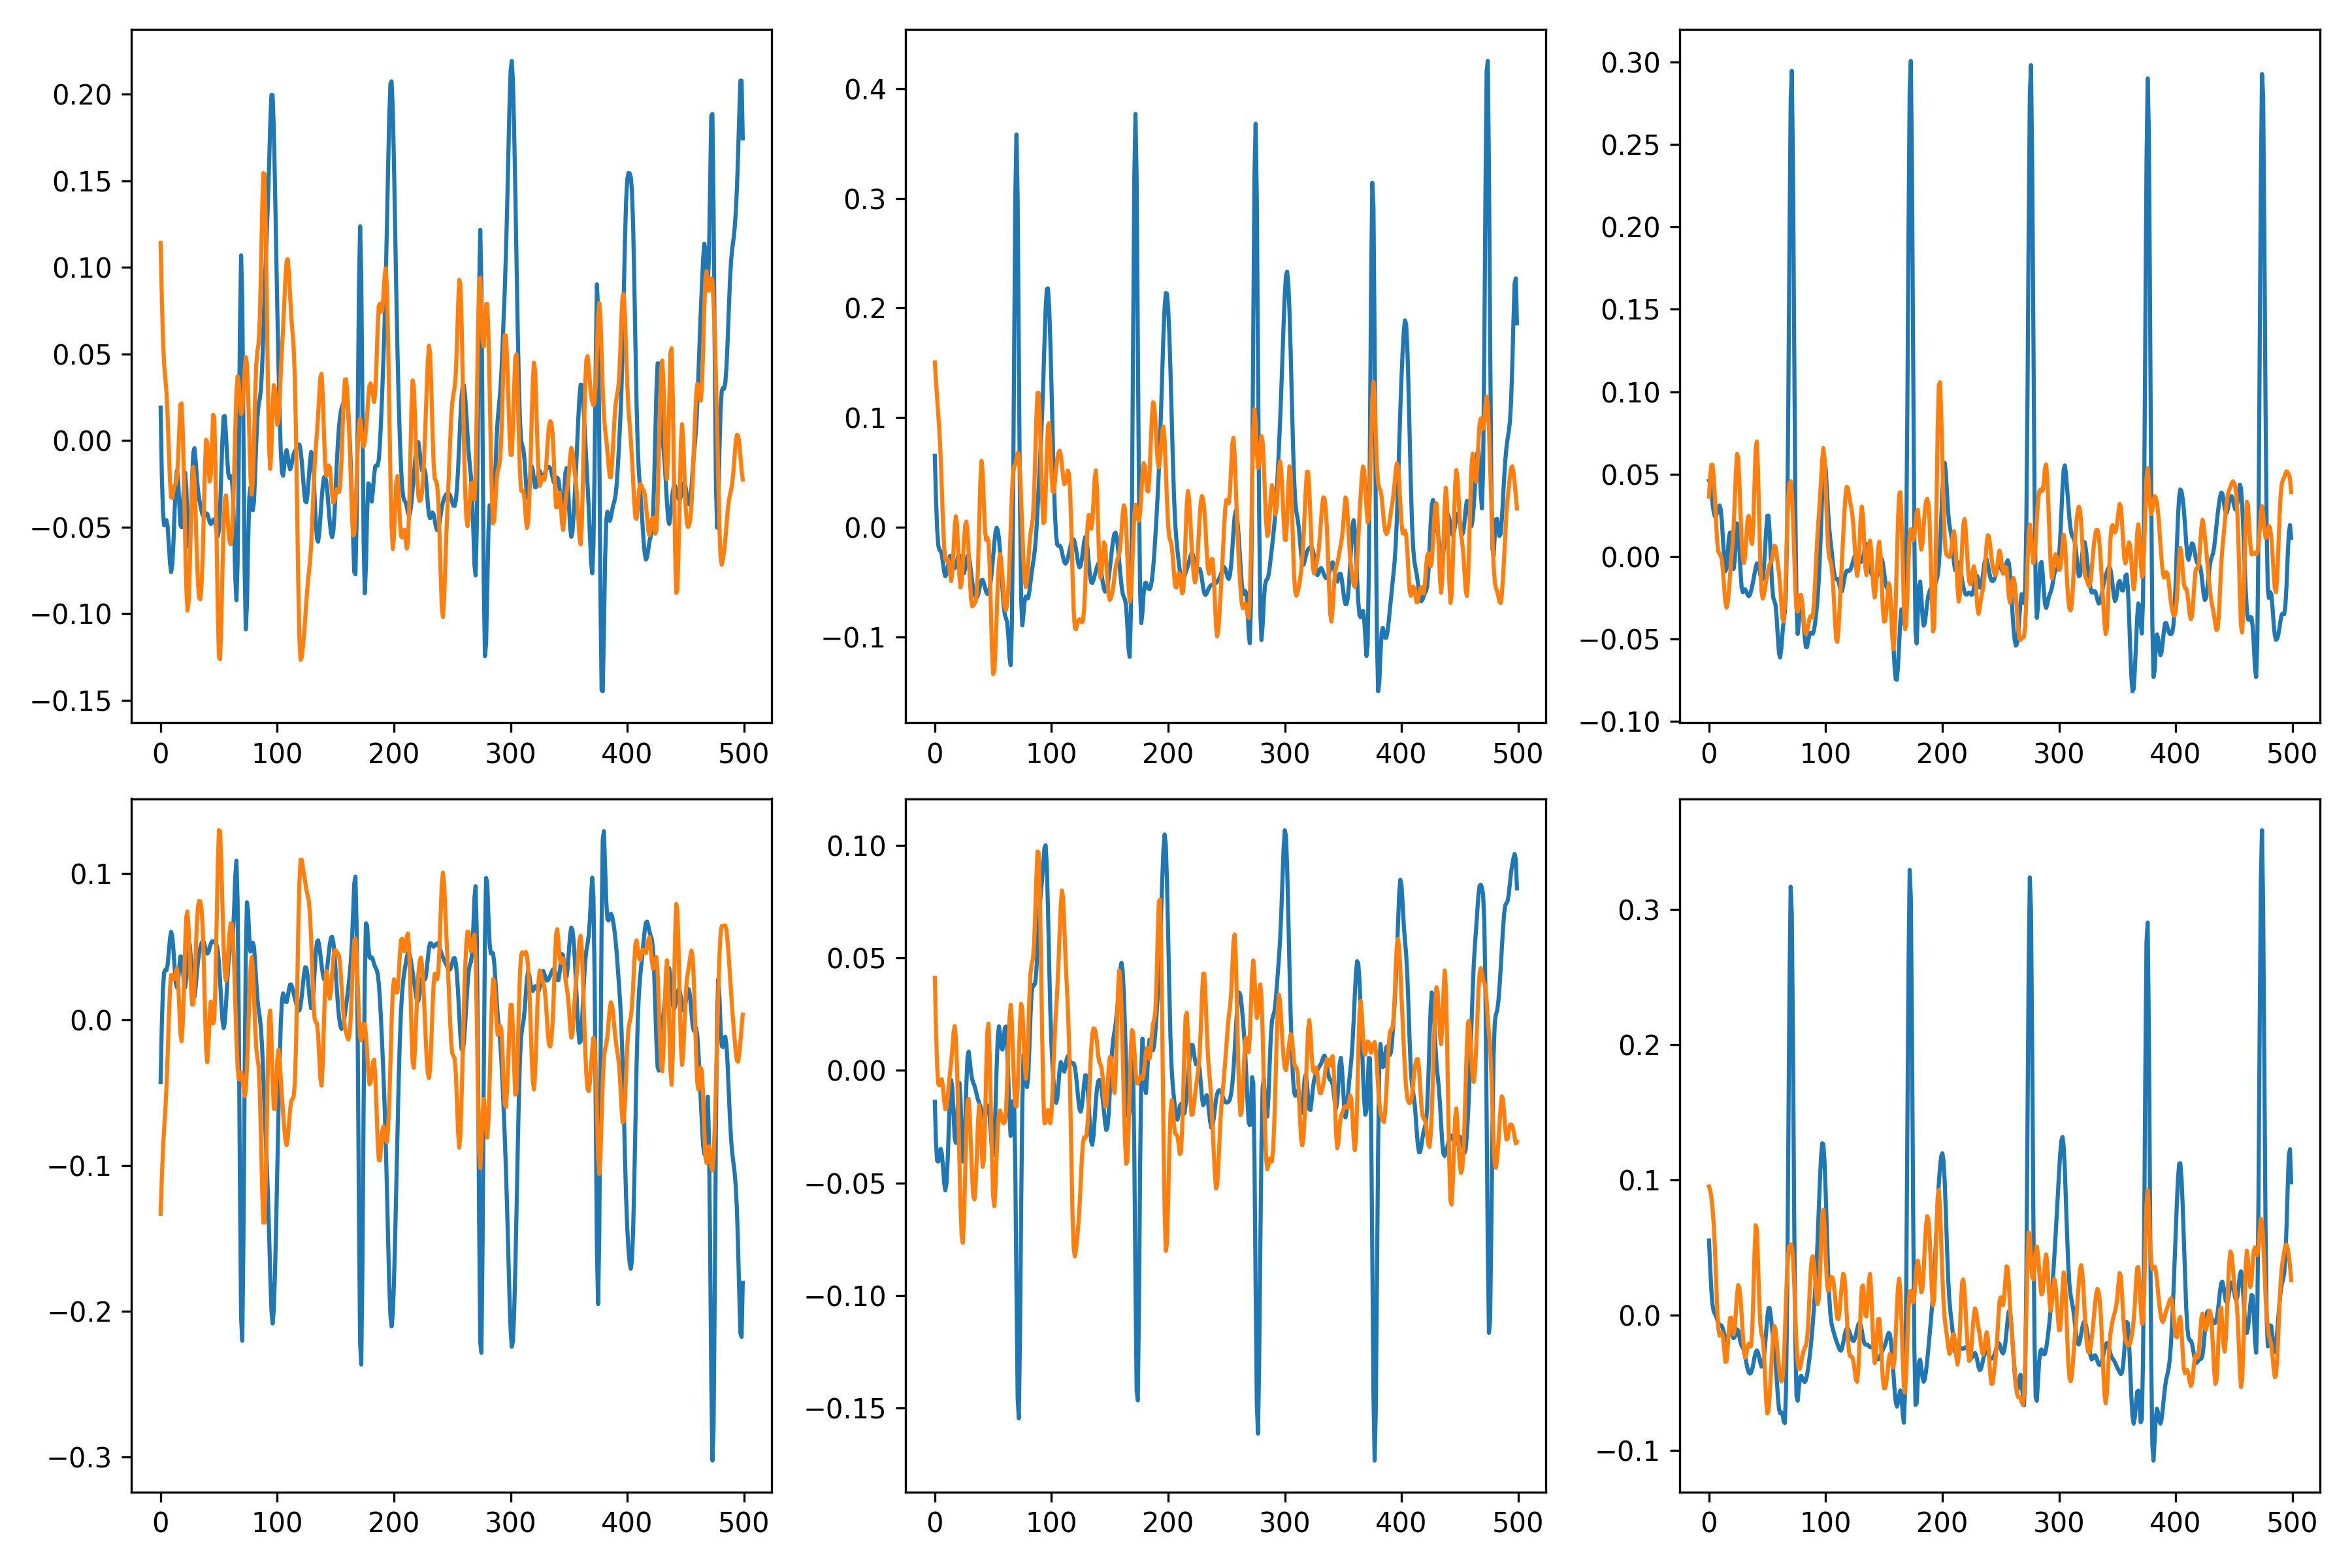
\includegraphics[width=0.85\textwidth]{images/first_cnn_result_second_plot_1.png}
    \captionsetup{justification=centering}
    \caption{Results obtained from the tests conducted after dataset simplification.}
    \label{fig:first_cnn_result_second_plot_1}
\end{figure}
\begin{figure}[H]
    \centering
    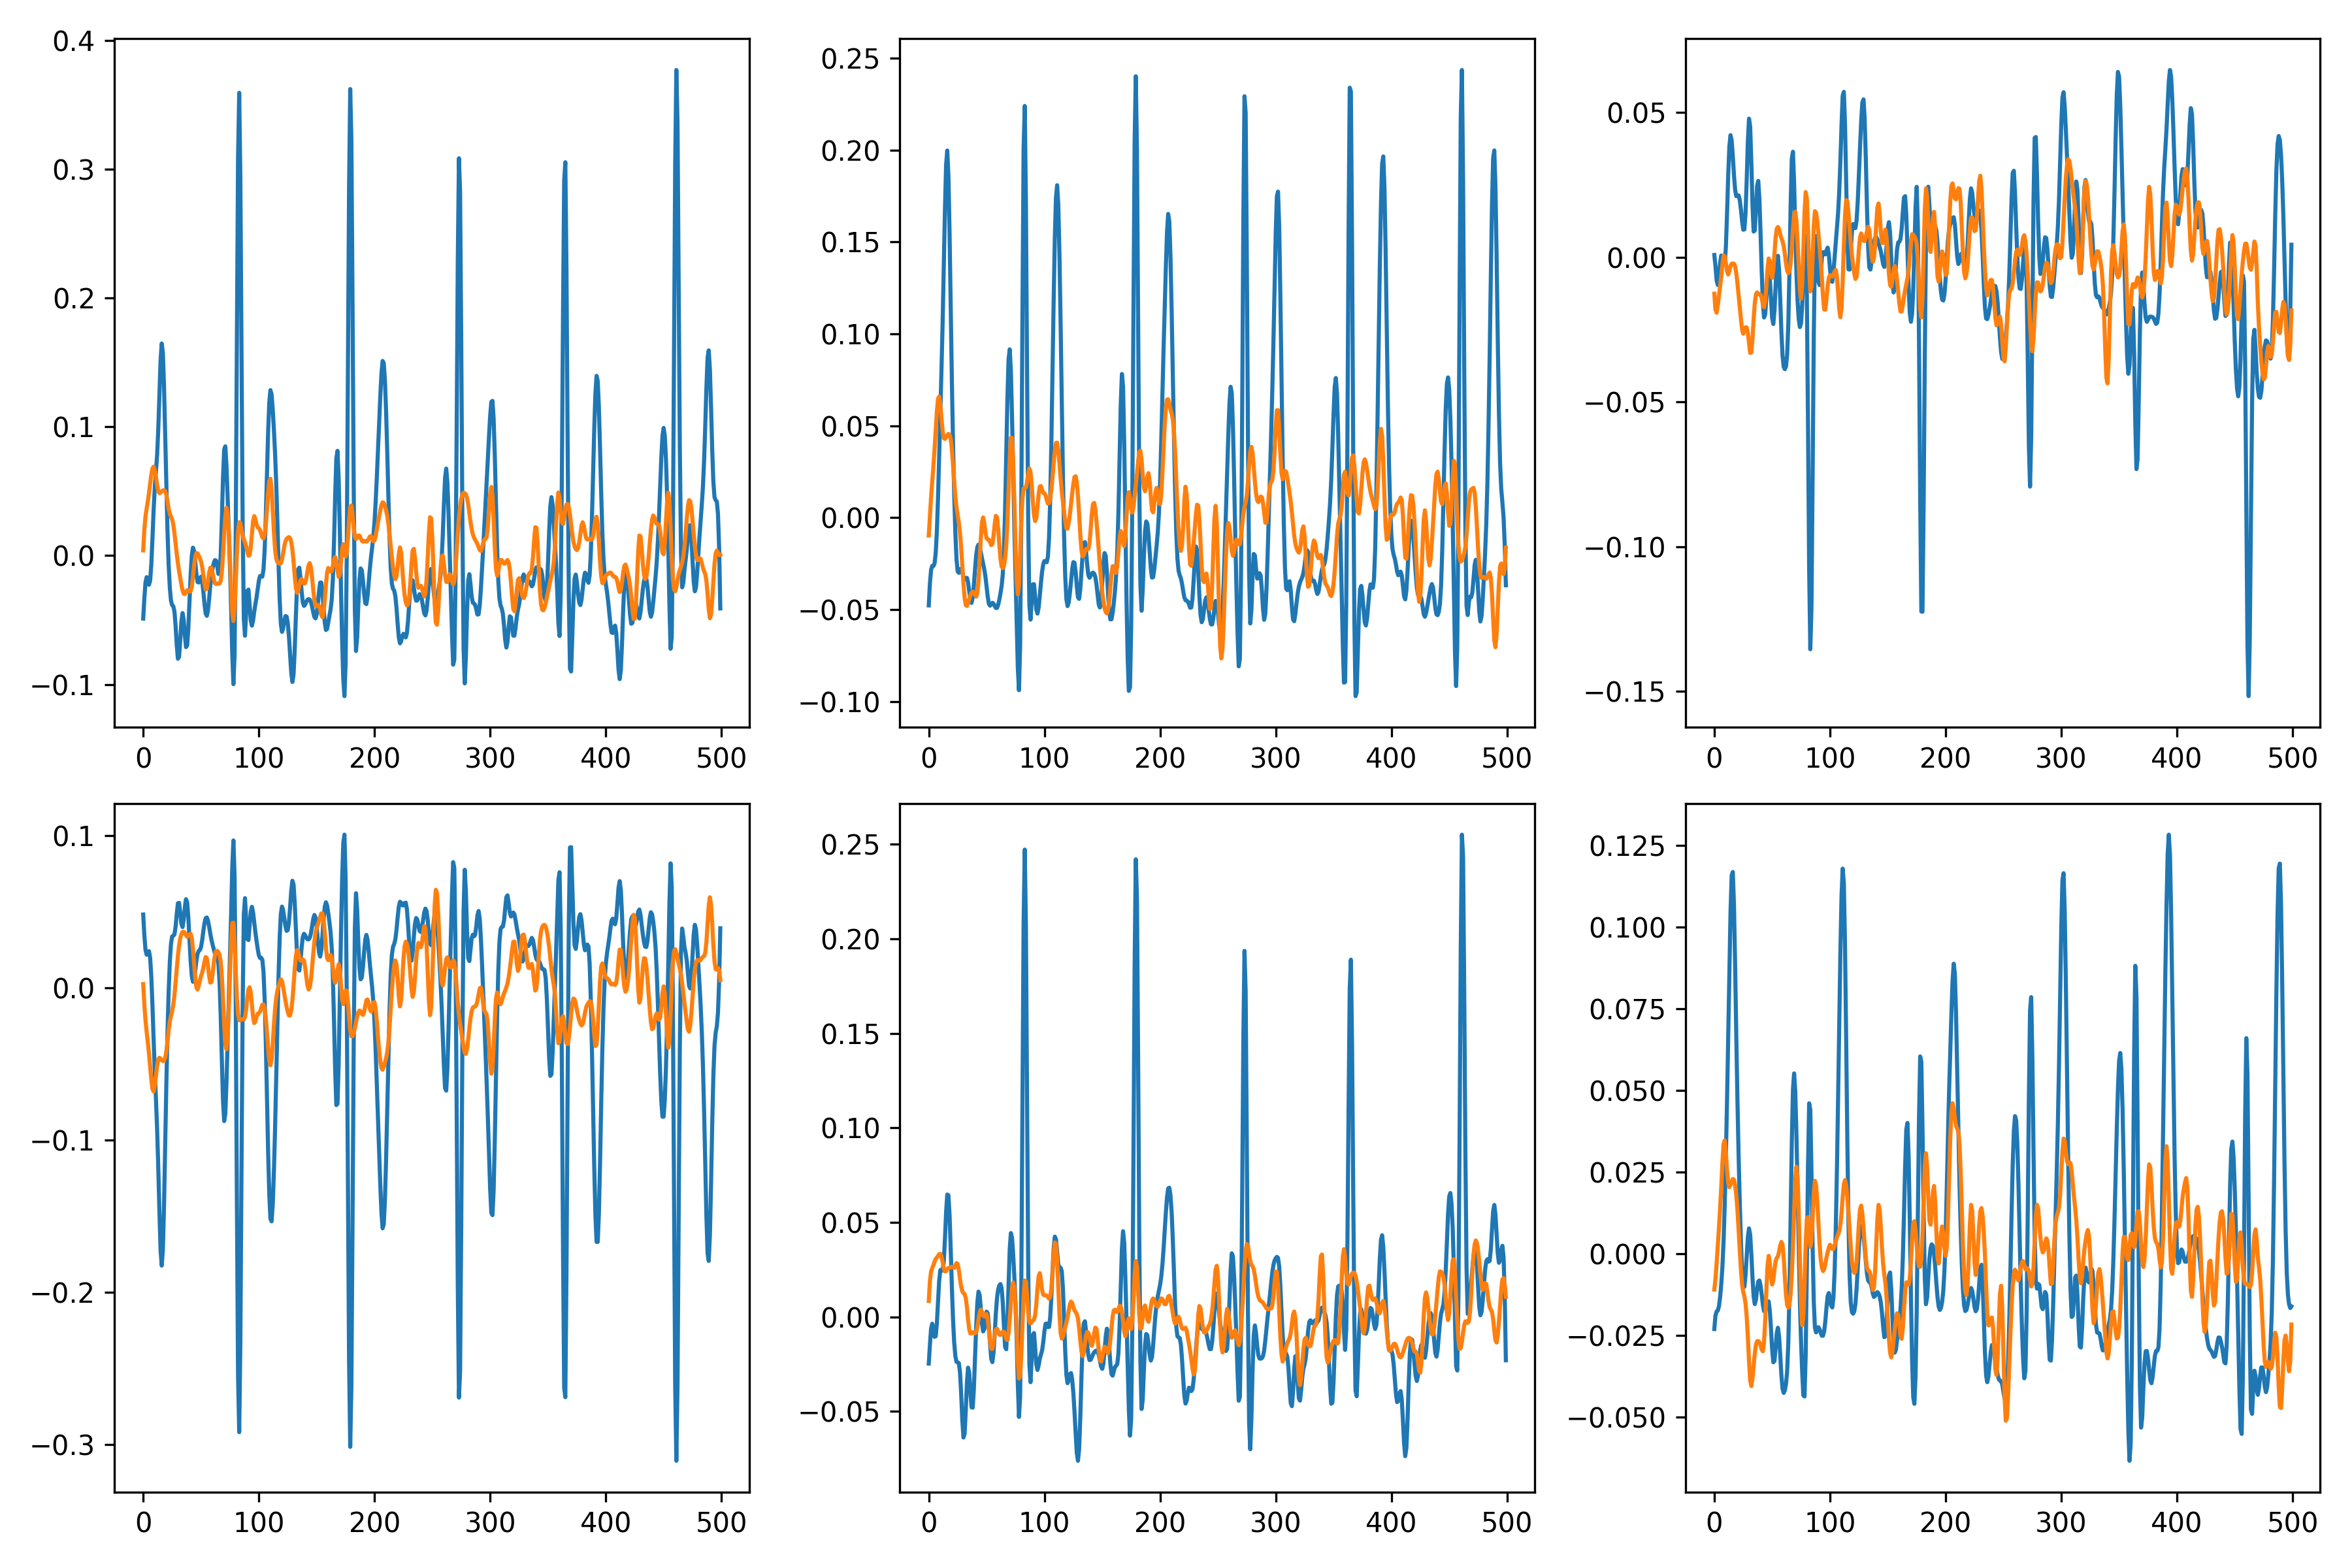
\includegraphics[width=0.85\textwidth]{images/second_cnn_result_second_plot_0.png}
    \captionsetup{justification=centering}
    \caption{Results obtained from the tests conducted after simplifying the dataset.}
    \label{fig:second_cnn_result_second_plot_0}
\end{figure}
\begin{figure}[H]
    \centering
    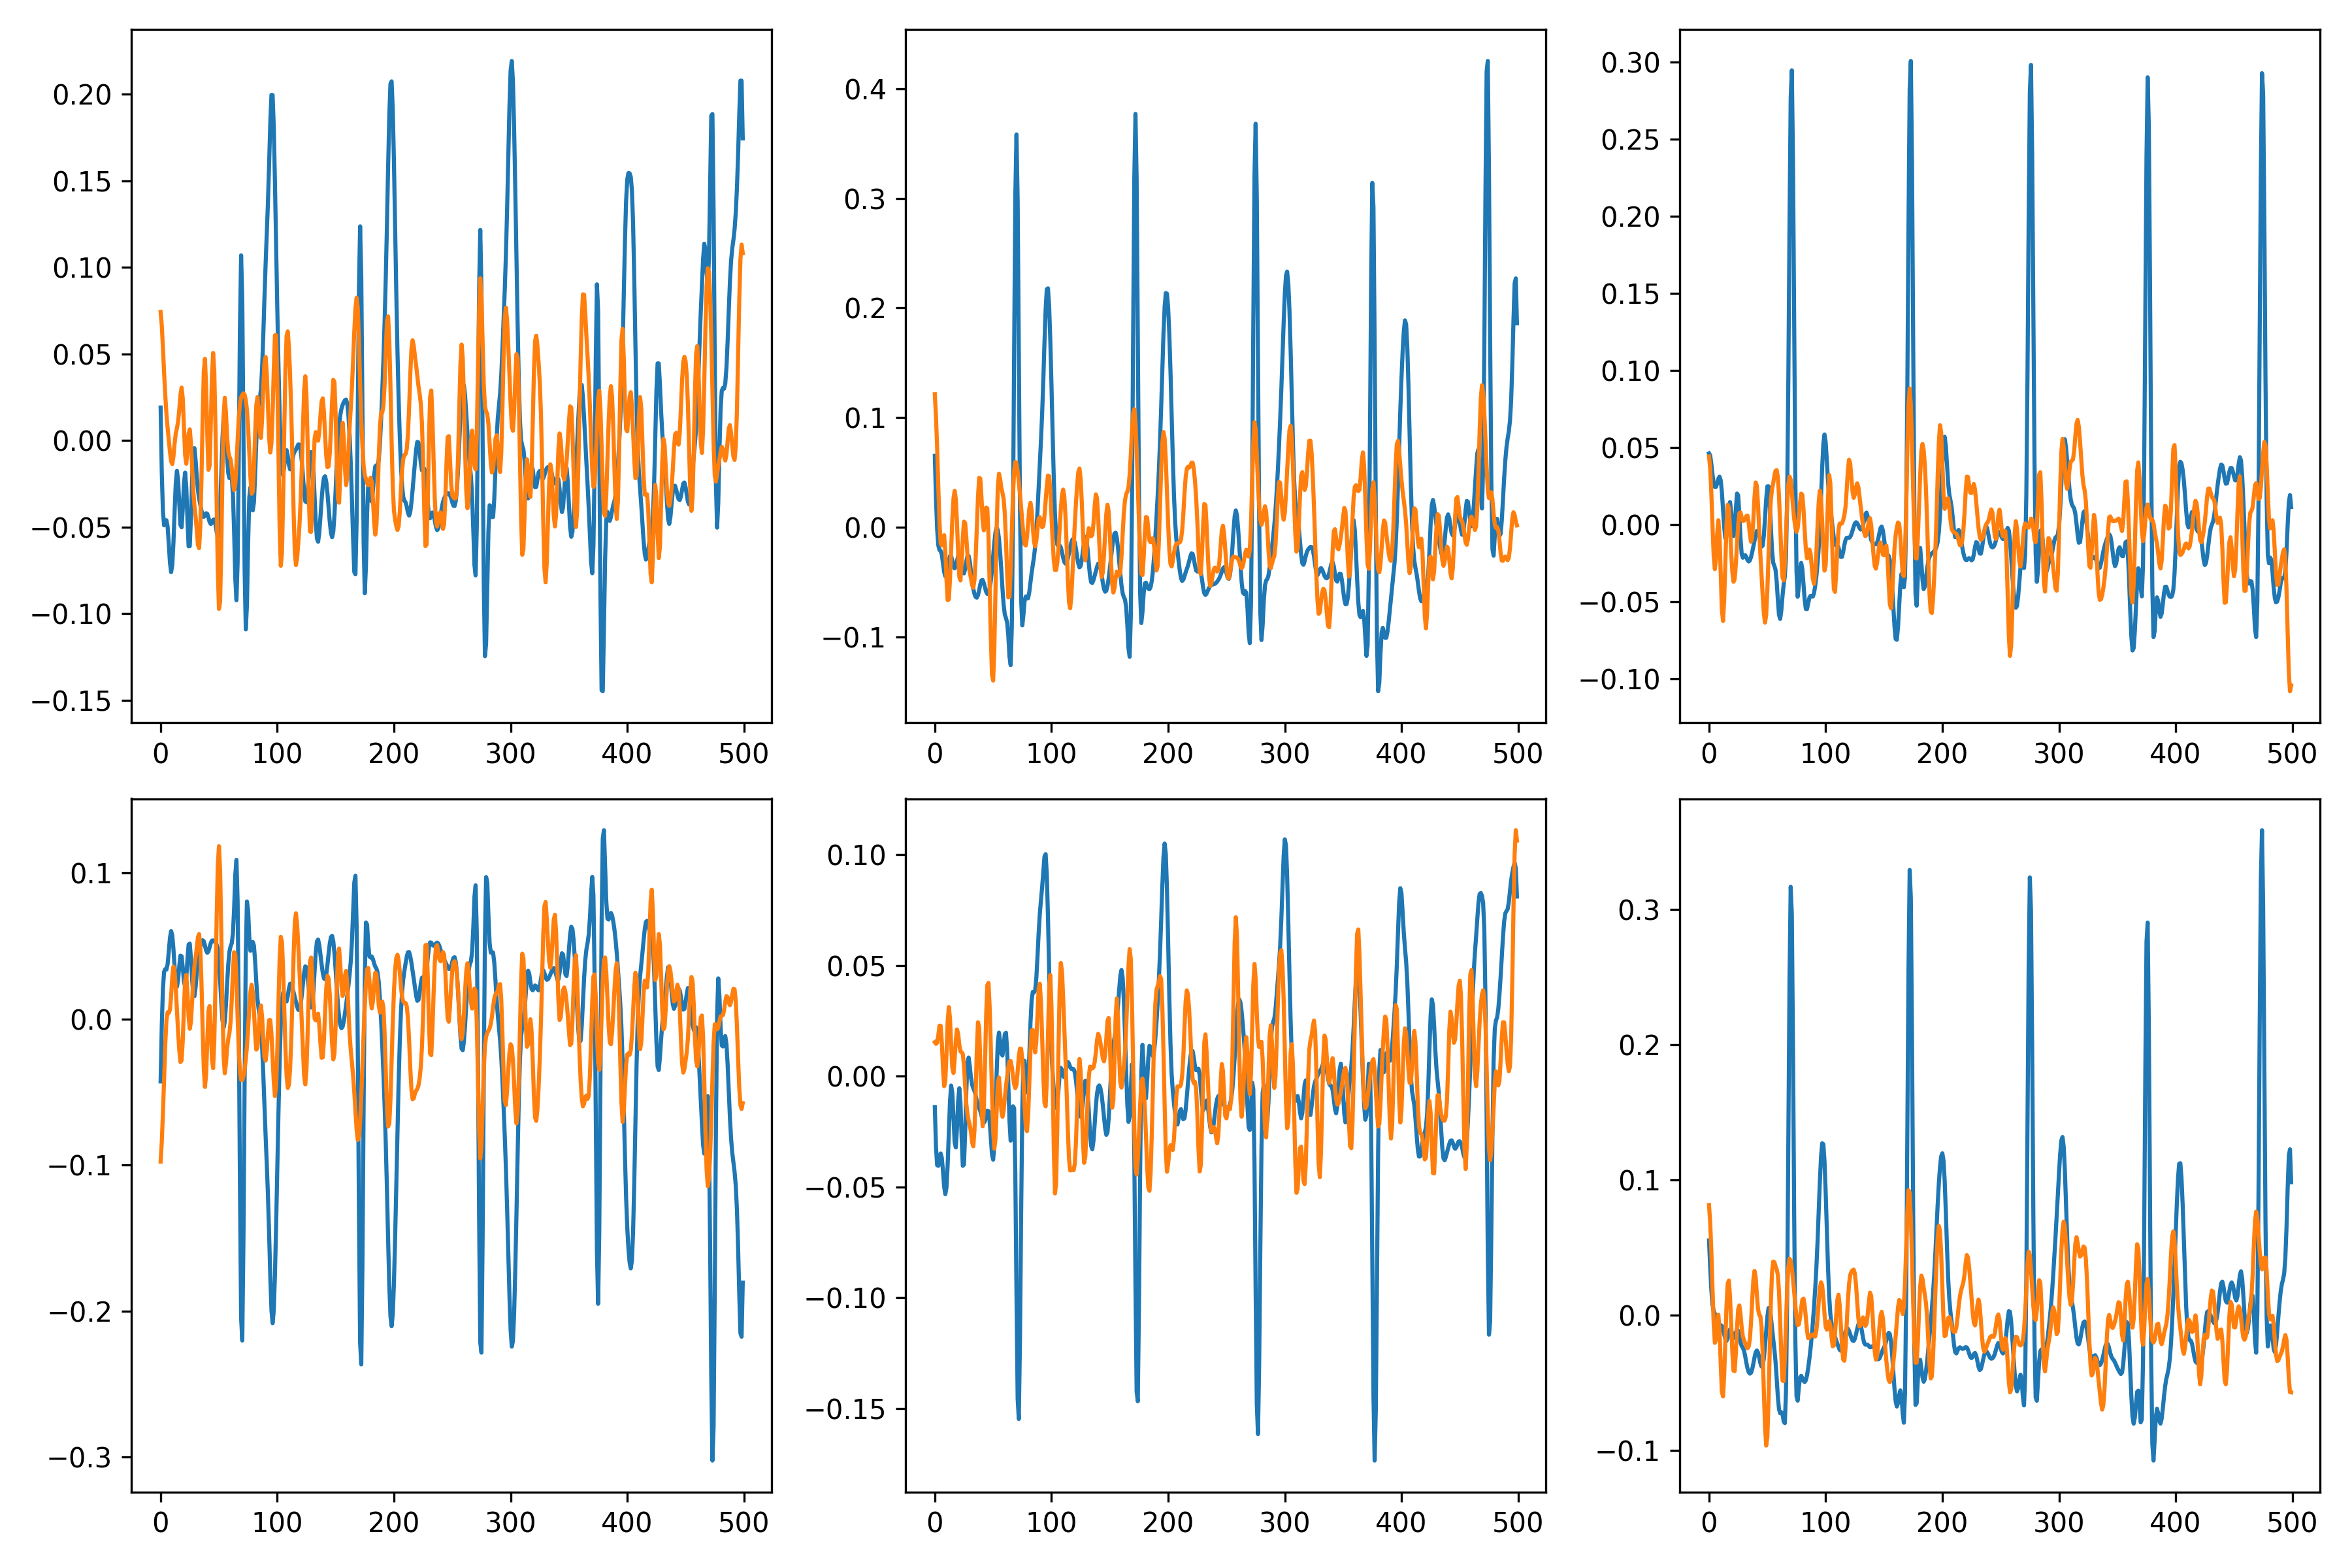
\includegraphics[width=0.85\textwidth]{images/second_cnn_result_second_plot_1.png}
    \captionsetup{justification=centering}
    \caption{Results obtained from the tests conducted after simplifying the dataset.}
    \label{fig:second_cnn_result_second_plot_1}
\end{figure}

\section{Discussion}
\label{sec:discussione}

As previously mentioned several times, unfortunately, the results obtained during the months of research testing were not satisfactory and did not meet the expectations initially hoped for. However, it is important to emphasize that in the use of deep learning, achieving optimal results immediately is never guaranteed. This situation is not unique in the field of deep learning: often, numerous tests and experiments are necessary to find the optimal configuration that leads to the desired results.

Nevertheless, a consistent and significant entropy result compared to expectations was achieved. The measured entropy effectively reflects the data's degree and provides a quantitative measure of the complexity of the studied system. This result confirms the validity of the adopted methodological approach and provides further evidence of the robustness of the analyses conducted.

Finally, regarding the three CNNs mentioned in the "Convolutional Neural Network" section (Chapter \ref{chap:materials}, Section \ref{sec:network}), the fact that none of them, including those not explicitly reported, yielded acceptable results does not pose a unique problem: it is an intrinsic characteristic of deep learning. The training process of neural networks can be influenced by various factors, including the complexity of the problem, the size and quality of the dataset, the choice of neural network architecture, and training parameters. Throughout the research period, numerous different neural network architectures were implemented and tested, and various hyperparameter configurations were explored to improve performance. However, despite the efforts and systematic approach, the results obtained did not fully meet expectations.

Of particular note was the complexity gap observed among all CNNs, especially among the three mentioned above, "simple," "intermediate," and more "articulate," which raises questions about why none of them brought clear and substantial improvements in results.

This observation was further emphasized following the application of the clustering algorithm, as despite the focus on working with ECGs that are similar through complexity reduction, none of the tested networks produced the desired results.

In conclusion, the research and experimentation process inherently involves trial and error, and success is not guaranteed in advance. It is crucial to consider the results as an integral part of the research process itself: indeed, this experience provided valuable insights, improved understanding of the problem under study, and paved the way for further research and developments regarding this issue.

\chapter{Conclusions}
\label{chap:conclusions}

Electrocardiography and \textit{deep learning} are nowadays an increasingly relevant combination and increasingly subject to being used in practice to improve precision and efficiency in the diagnosis and classification of cardiac conditions.

On the other hand, the flip side concerns the lack of adequate datasets for training the networks, as well as the lack of precise and adequate evaluation procedures capable of ensuring the similarity of different algorithms. Indeed, one of the main aspects in the application of \textit{deep learning} to ECG analysis is the availability of large and high-quality training datasets: collecting and annotating these datasets still represents a significant challenge that requires considerable human effort and collaboration between doctors and researchers.

Despite these challenges, the results obtained so far are extremely promising: the combination of medical expertise and \textit{deep learning} knowledge is opening up new perspectives, and the use of \textit{deep learning} in ECG analysis represents a rapidly evolving field that will certainly play an increasingly prominent role in clinical cardiology practice.

Standard ECGs consist of 12 leads used to record the electrical potentials of the heart's atria and ventricles. In this type of ECG, four electrodes are placed on the patient's limbs and six on the surface of the chest, so the overall electrical potential of the heart is measured in twelve point differences, commonly called "leads," and recorded for a predetermined period of time, usually ten seconds. Therefore, the correct interpretation of the ECG is possible with a high-quality 12-lead tracing, and it is advisable to follow a systematic approach that allows proceeding in a predefined order.

Electrocardiography allows the detection of many cardiac conditions but is also used for continuous monitoring of cardiac patients, recording the heart's electrical activity and allowing detailed evaluation.

In relation to 12-lead ECGs, Frank leads are of fundamental importance, representing a methodology of electrocardiographic acquisition that provides detailed information on the spatial distribution of cardiac electrical activity. Unlike standard 12-lead ECGs, Frank leads allow for a more complete mapping of cardiac electrical activity, enabling a different evaluation of the morphology of electrical impulses as well as cardiac anomalies and disorders.

The aim of the research was to reconstruct, based on an ECG, the signal that would ideally follow it over time. Since paper ECGs are still widely used in clinics and have a duration of ten seconds, with the first five showing the first 6 leads of the ECG and the remaining five showing the remaining 6 leads, the goal was to reconstruct the leads that are not observed, namely the first 6 in the second five seconds and the second 6 in the first five seconds.

The dataset used in the research was identified in \textit{PTB-XL}, an extensive dataset of ECGs developed in Germany containing recordings of high-resolution signals, both 12-lead and 15-lead. The dataset includes ECGs from healthy patients as well as from patients with cardiac abnormalities, totaling 21,799 12-lead ECGs from 18,869 patients, each lasting 10 seconds. Additionally, the dataset is integrated with detailed metadata on demographics, infarction characteristics, diagnostic statement probabilities, and reported signal properties. During the publication process in 2019, the dataset was optimized with particular attention to usability and accessibility for the \textit{deep learning} community, ensuring that the data can be easily processed by standard software.

However, since the dataset also includes ECGs from patients with cardiac abnormalities, it was first necessary to filter the signals to work exclusively with ECGs from healthy patients.

During the research, many initially unexpected problems emerged, requiring efforts to find ways to achieve the desired results. One of these was applying entropy calculation, which provides a basis for decision-making, optimization, and understanding of the problem to be solved.

To perform the actual reconstruction of ECGs, several convolutional neural network models were introduced, implemented, tested, and adapted multiple times in search of good results. In particular, networks were implemented and grouped into three distinct types: simple networks consisting solely of a set of convolutional layers, networks consisting of this same set of layers combined with an external component introduced to address performance degradation, and finally, much more elaborate networks consisting of multiple intertwined components operating in unison. Unfortunately, none of these types yielded the desired results, as verified through observation and the \texttt{MSE} function, short for \textit{Mean Squared Error}. However, it was very useful to implement and test networks of such varying complexity incrementally to observe how results evolved and changed over time during testing.

However, after verifying once again the unsatisfactory results from all implemented CNNs, the idea was to simplify the data as much as possible for training by adopting the \textit{K-means} clustering algorithm to group ECGs with similar characteristics into different clusters. In this way, ideally, CNNs should produce better results due to the similarity among signals while still maintaining a significant total number, crucial for proper network training.

Through an in-depth analysis carried out throughout the entire research period, significant results were obtained that contribute to understanding how complex and non-trivial it is to achieve satisfactory results within the limited time dedicated to thesis work, conducting a finite number of tests that do not always yield fortuitous results. However, it is important to note that this research has some limitations, such as those of a temporal nature and those related to the dataset used, related to data quality and extensive size, which required significant time for execution and testing. Nevertheless, this work represents a step forward in the reconstruction of electrocardiographic signals and provides interesting insights for future investigations and research. Therefore, it can be confidently stated that this research has strongly emphasized the importance of using AI and \textit{deep learning} and provides a solid foundation for further explorations in a field that is evolving rapidly day by day.

\afterpage{\blankpage}

\bibliographystyle{unsrt}
\bibliography{bibliography}
\addcontentsline{toc}{chapter}{Bibliography}

\afterpage{\blankpage}

\end{document}